%&latex
\documentclass[10pt,fleqn]{article} \pdfoutput=1

\addtolength{\oddsidemargin}{-.875in}
\addtolength{\evensidemargin}{-.875in} \addtolength{\textwidth}{1.75in}

\addtolength{\topmargin}{-.875in} \addtolength{\textheight}{1.75in}

\openup 1em

%macro for commenting
\usepackage{color}

\newcommand{\leo}[1]{{\color{blue}{#1}}}
\newcommand{\alex}[1]{{\color{red}{Alex: #1}}}
\newcommand{\aki}[1]{\color{green}{Aki: #1}}

% \newcommand{\Xbeta}{ X_i \theta}
\newcommand{\xbeta}{ x_i \beta} \newcommand{\xtheta}{ x_i \theta}
% \newcommand{\xbetaij}{ x_{ij}^T \theta}
\newcommand{\sgamma}{s_{ij}^T\gamma_i} \newcommand{\core}{\textbf{CORE}}

\usepackage[round]{natbib}

\usepackage{rotating} \usepackage{graphicx} \usepackage{subcaption}

\usepackage{float} \usepackage{bbm}

\usepackage{amsthm,amsmath, amssymb} \usepackage{mathrsfs}
\usepackage{subcaption}
%\usepackage{nicefrac}


\newtheorem{theorem}{Theorem} \newtheorem{lemma}{Lemma}
\newtheorem{corollary}{Corollary} \newtheorem{remark}{Remark}
\newtheorem{example}{Example} \newtheorem*{Hausdorff_def}{Definition -
Hausdorff Measure}


\usepackage{algorithm} \usepackage{algpseudocode} \usepackage{array}

%\usepackage{mhequ}
\newcommand{\be}{\begin{equation}\begin{aligned}}
\newcommand{\ee}{\end{aligned}\end{equation}}
\newcommand{\bb}[1]{\mathbb{#1}} \newcommand{\mc}[1]{\mathcal{#1}}
\DeclareMathOperator{\Binom}{Binomial} \DeclareMathOperator{\No}{No}
\DeclareMathOperator{\PG}{PG} \DeclareMathOperator{\IG}{Inverse-Gamma}
\DeclareMathOperator{\Ga}{Gamma} \DeclareMathOperator{\Bern}{Bernoulli}
\DeclareMathOperator{\U}{Uniform} \DeclareMathOperator{\Poi}{Poisson}
\DeclareMathOperator{\NB}{NB} \DeclareMathOperator{\cov}{cov}
\DeclareMathOperator{\var}{var} \DeclareMathOperator{\diag}{diag}
\DeclareMathOperator{\Diag}{Diag}
\newcommand{\KL}[2]{\textnormal{KL}\left(#1 \parallel #2\right)}
\DeclareMathOperator{\1}{\mathbbm{1}} \DeclareMathOperator{\bigO}{\mc O}
\newcommand{\dt}{\epsilon} % Stepsize of leapfrog
\newcommand{\mass}{M} %Mass matrix 
\newcommand{\hess}{\mathbf{H}} % Hessian notation.



\thispagestyle{empty} \baselineskip=28pt

\title{\textbf{Constraint Relaxation for Bayesian Modeling with Parameter
Constraints}}
\author{Leo L Duan, Alexander L Young, Akihiko Nishimura, David B Dunson} 

\date{}
\begin{document}

\maketitle {\bf Abstract:}

Prior information often takes  the form of parameter constraints. Bayesian
methods include such information through prior distributions having constrained
support. By using posterior sampling algorithms, one can quantify uncertainty
without relying on asymptotic approximations. However, outside of narrow
settings, \leo{the choices of priors and efficient sampling algorithms are
severely limited.  } Motivated to addresses these problems, we propose to
relax the parameter support into the neighborhood surrounding constrained
space. \leo{ This allows us to utilize the much larger family of prior
distributions and off--the--shelf sampling algorithms available in general
unconstrained space.  The relaxed model can be directly used for statistical
inference, or viewed as an approximate solution to the original constrained
problem. We study the constrained and relaxed distributions under multiple
settings, and theoretically quantify their differences. Popular state--of--art
sampling algorithms such as leap-frog Hamiltonian Monte Carlo can be directly
utilized with almost no customization.} We illustrate this approach through
multiple novel modeling examples involving equality and inequality constraints.

\vskip 12pt
	%\baselineskip=12pt \par\vfill\noindent
	{\noindent KEY WORDS: Constrained Bayes, Constraint
	Functions, Shrinkage on Manifold, Support Expansion, Ordered Simplex}
%\par\medskip\noindent \clearpage\pagebreak\newpage
\pagenumbering{arabic}

\newpage

\section{Introduction}

It is extremely common to have prior information available on parameter
constraints in statistical models. For example, one may have prior
knowledge that a vector of parameters lies on the probability simplex or
satisfies a particular set of inequality constraints. Other common examples
include shape constraints on functions, positive semi-definiteness of
matrices and orthogonality. There is a very rich literature on optimization
subject to parameter constraints. One common approach is to rely on Lagrange
and Karush-Kuhn-Tucker multipliers \citep{boyd2004convex}. However, simply
producing a point estimate is often insufficient, as uncertainty
quantification (UQ) is a key component of most statistical analysis. Usual
large sample asymptotic theory, for example showing asymptotic normality of
statistical estimators, tends to break down in constrained inference
problems. Instead, limiting distributions may have a complex form that
needs to be re-derived for each new type of constraint, and may be
intractable.

An appealing alternative is to rely on Bayesian
methods for UQ, including the constraint through a prior distribution
having restricted support, and then applying Markov chain Monte Carlo
(MCMC) to avoid the need for large sample approximations. \leo{
This strategy appears conceptually simple, however, except for a few limited cases,
it is generally very difficult to find appropriate prior distribution in constrained space and
to develop tractable posterior sampling algorithm.}

To overcome these difficulties, one common strategy  is to reparameterize
with un-/less constrained parameters at equal or less dimension. The
new parameters form functions that can always satisfy the constraint. The
transformation is known as `coordinate system' in manifold embedding literature
\citep{nash1954c1,do2016differential}. Examples include the polar coordinates
for a unit sphere, or stick-breaking construction for Dirichlet distribution on
probability simplex \citep{ishwaran2001gibbs}.  One can then directly assign
prior on the less constrained parameters. \leo{Despite a few successes, in
general, it is difficult to assign prior on the new parameterization while preserving property on the original constrained space. For example, uniformity on a compact constrained space often
requires a non-uniform distribution based on the new parameterization, which
can be intractable (See \cite{diaconis2013manifold} for details). Moreover,
convenient reparameterzation does not always exist, especially when multiple
constraints are involved.}

As a result, the solutions are often limited to a few distributions for
specific constraints. For example, for modeling of data on Stiefel manifolds,
one routinely relies on von Mises-Fisher and matrix Bingham-von Mises-Fisher
distributions \citep{khatri1977mises,hoff2009simulation}, \leo{ which are
both derived from constrained Gaussian}. \leo{Often, the flexibility of these distributions
is questionable in accommodating the modern complexity of data, such as
possible sparsity, presence of outlier, multi-modality, etc.. Motivated
to address this issue, non-parametric Bayes approach has been exploited
to extend the flexibility, such as the work by
\cite{lin2016bayesstiefel} on Stiefel manifold; although such cases are rare for other constraints.}

\leo{
Besides the modeling difficulty, posterior sampling has been another
challenge under parameter constraint.} Early work \citep{gelfand1992bayesian}
suggested using general unconstrained distribution inside a simple
truncated space, and running Gibbs sampling ignoring the constraint but
only accepting the draws that fall into truncated space. Unfortunately,
this method can be highly inefficient if constrained space has a small or
zero measure, which will create a low or zero acceptance probability. A
recent idea is to run MCMC ignoring the constraint, and then project draws
from the unconstrained posterior to the appropriately constrained space.
Such an approach was proposed for generalized linear models with order
constraints by \cite{dunson2003bayesian}, extended to functional data with
monotone unimodal constraints \citep{gunn2005transformation}, and recently
modified to nonparametric regression with monotonicity \citep{lin2014monogp}
or manifold \citep{lin2016extrinsic} constraints. Another direction utilizes
a customized Hamiltonian Monte Carlo (HMC) with geometric flow for a few
selected constraints \citep{byrne2013geodesic}.  \leo{On the other hand,
those approaches are arguably highly customized, which cannot directly exploit the rapidly developing automatic tools such as STAN \citep{carpenter2016stan}.}

\leo{The goal of this article is to dramatically simplify the constrained modeling
problem, by {\em relaxing} the parameter into the
neighborhood surrounding the constrained space. One could exploit the
larger family of prior distributions and off--the--shelf sampling
algorithms available in general unconstrained space.
Due to the proximity to the constrained space, the relaxed model enjoy
property similar to the constrained model, such as an improved convergence
in latent factor model as shown in data application. Alternatively, one
could view the collected posterior samples as approximation to ones under
constrained model. We carefully quantify the difference in the theoretic study.
}


\section{Constraint Relaxation Methodology}

In conventional models under constraints, assume that $\theta$ is an
$\mathcal{R}$-valued random variable with dimensionality
$\dim(\mathcal{R})=r<\infty$ and that $\theta$ is subject to some
constraints restricting it to a subset $\mathcal{D} \subset \mathcal{R}$.
In Bayesian setting, $\theta$ is a parameter where constraints arise from
some given information.

As a motivating example, consider the case where $\theta$ has prior density
$\pi_\mathcal{D}(\theta)$ with support on $\mc D$. The posterior density of $\theta$
given data $Y$ and $\theta \in \mathcal{D}$ is,

\begin{equation*}
\pi_{\mc D}(\theta \mid  Y) \propto \mathcal{L}(\theta; Y)
\pi_\mathcal{D}(\theta) .
\end{equation*}

There are two primary problems motivating this work: the choice of
$\pi_{\mc D}$ is very limited, which severely restricts the scope of modeling; posterior sampling often is difficult. To address these challenges, we consider an
alternative model that {\em relaxes} the constraints by placing a high
probability in the neighborhood of $\mathcal{D}$ but has support in $\mathcal{R}$. Suppose we used the density

\begin{equation}
\label{EQ:Rel_Dens_Motivation}
\tilde{\pi}(\theta) \propto
\mathcal{L}(\theta; Y)  \pi_\mathcal{R}(\theta)
\exp\bigg(-\frac{1}{\lambda} \|v_\mathcal{D}(\theta)\|\bigg)
\end{equation}
where  $\pi_{\mc R}(\theta)$ is proportional to $\pi_{\mc D}(\theta)$ without
the constraint, i.e. $\pi_\mathcal{D}(\theta) \propto \pi_\mathcal{R}(\theta)
\mathbbm{1}_{\mc D}(\theta)$. We assume $\pi_{\mc R}(\theta)$ is proper, so
that the posterior is proper as well. We use $\|v_\mathcal{D}(\theta)\|$ as
a distance from $\theta$ to the constrained space (e.g. $\inf_{x\in\mathcal{D}}
\|\theta-x\|_2$ with $\|.\|$ an appropriate metric).

Note that $\mathbbm{1}_\mathcal{D}(\theta)$ is the pointwise limit of
$\exp\big(- \lambda^{-1}\|v_\mathcal{D}(\theta)\|)$ (except perhaps on the
boundary of $\mathcal{D}$) as $\lambda \to 0^+.$ However, (1) has
support $\mathcal{R}$ for all $\lambda > 0$, hence `relaxing' the
constraint. As shown in later sections, the immediate benefits are that one
could use general unconstrained prior for $\pi_{\mc
R}(\theta)$, and posterior sampling becomes much simpler.
We refer to this strategy as Bayes constraint relaxation (\core).

We investigate a number of questions about Bayes CORE:  (i) For
what types of distributions and constraints is CORE suitable? (ii) Is there
a general approach for constructing the `relaxed' distribution? (iii) How
well do samples from the relaxed model approximate the
original constrained distribution?  (iv) How does the amount of relaxation depend on the tuning parameter $\lambda$?

The answers to (ii) - (iv) depend largely upon (i).  Therefore, beginning with
(i), we assume $\theta$ is a continuous random variable (e.g.  $\mathcal{R}$
is $[0,\infty)^d$, $\mathbb{R}^{n\times k}$) and  $\pi_{\mc R}(\theta)$ is
absolutely continuous with respect to Lebesgue measure on $\mathcal{R}$ hereby
denoted as $\mu_\mathcal{R}$. We investigate two general types of constraints.

\subsection{Constrained Space with Positive Measure}
\label{SEC:Positive_measure_methods}

We first consider the simpler case where $\mathcal{D}$ has positive measure,
i.e.  $\int_\mathcal{D} {\mc L}(\theta;y)\pi(\theta)d\mu_\mathcal{R}(\theta)
>0$.  Generally, inequality constraints (e.g.  $a^T\theta
< 0$, $\|\theta\|_2^2 < 1$) fall into this category.

The constrained posterior density is a result of simple
renormalization:

$$\pi_\mathcal{D}(\theta\mid Y) = \frac{\mathcal{L}(\theta; Y)
\pi_\mathcal{R}(\theta)\mathbbm{1}_\mathcal{D}(\theta)}{\int_\mathcal{D}
\mathcal{L}(\theta; Y)
\pi_\mathcal{R}(\theta)d\mu_\mathcal{R}(\theta)}\propto \mathcal{L}(\theta;
Y) \pi_\mathcal{R}(\theta)\mathbbm{1}_\mathcal{D}(\theta), $$
which is defined with respect to $\mu_\mathcal{R}$.

We now consider a relaxed density
\begin{equation}
\label{EQ:relaxedDensityPosMeasure}
\tilde{\pi}_\lambda(\theta) =
\frac{\mathcal{L}(\theta;
Y)\pi_\mathcal{R}(\theta)\exp\big(-
\lambda^{-1}{\|v_{\mc
D}(\theta)\|}\big)}{\int_{\mathcal{R}}\mathcal{L}(\theta; Y)
\pi_\mathcal{R}(\theta)\exp\big(-{\lambda^{-1}}{\|v_{\mc
D}(\theta)\|}\big)
d\mu_\mathcal{R}(\theta)} \propto
\mathcal{L}(\theta; Y)
\pi_\mathcal{R}(\theta)\exp\big(-{\lambda^{-1}}{\|v_{\mc
D}(\theta)\|}\big)
\end{equation}
which is also absolutely continuous with respect to $\mu_\mathcal{R}.$
Here $\lambda >0$ and $v_{\mc
D}(\theta)$ is a scalar-valued function which measures
the distance
from $\theta$ to the constrained space $\mathcal{D}$, i.e.  $v_{\mc
D}(\theta) = 0 \quad \forall \theta \in \mathcal{D}$
and is
positive otherwise.  Formally, as $\lambda \to 0^+$, $\exp(-v_{\mc
D}(\theta)/\lambda) \to \mathbbm{1}_\mathcal{D}(\theta)$ pointwise.
If $\mathcal{D}$ is an open subset of $\mathcal{R}$, this limit may not hold
on the boundary of $\mathcal{D}$, denoted $\partial
\mathcal{D}$; however in general, $\mu_\mathcal{R}(\partial
\mathcal{D}) = 0$.

There are many possible choices for $\|v_{\mathcal D}\|$ which may be selected
for different reasons.  Perhaps the most intuitive choice is to take

$$
\|v_{\mc D}(\theta)\| =
\inf_{x\in\mathcal{D}} \|\theta-x\|_k
\qquad	\text{ or }
\|v_{\mc D}(\theta)\| = \inf_{x\in\mathcal{D}}
\sqrt{(x-\theta)^T A (x-\theta)}$$
where $\|\cdot\|_k$ denotes the distance using the $k$-norm, used
for isotropic relaxation; $A$ is positive definite for directional
relaxation. Alternatively, one may choose distance for convenient computation,
such as closed-form. For example, for inequality $\theta_1+\theta_2<0$,
one could use $\|v_{\mc D}(\theta)\|=\max(\theta_1+\theta_2,0)$. As long as
$\|v_{\mc D}(\theta)\|$ is zero for $\theta \in \mathcal{D}$ and positive
for $\theta\not\in\mathcal{D}$, it follows that $\pi_\mathcal{D}$ is the
pointwise limit of $\tilde{\pi}_\lambda$ for $\mu_\mathcal{R}$ a.e.  $\theta$
in $\mathcal{R}.$

One utility of CORE is to obtain approximate estimate
$\bb E[g(\theta) \mid \theta\in\mathcal{D}]$ via the relaxed
posterior density, $\tilde{\pi}_\lambda$. For small $\lambda$, it is
natural to anticipate

$$\int_\mathcal{R} g(\theta)\tilde{\pi}_\lambda(\theta)
d\mu_\mathcal{R}(\theta) \approx \int_\mathcal{D}
g(\theta)\pi_\mathcal{D}(\theta) d\mu_\mathcal{R}(\theta) .$$

Rigorous
details for its validity, a suitable class of
functions for which it applies and rates of convergence in $\lambda$ are
contained in Section \ref{SEC:Positive_measure_theory}. For now, we
illustrate a common case of modeling under linear inequality.

\textbf{Example: Constrained Gaussian  under Linear Inequality}

Suppose that $\theta = (\theta_1,\theta_2)\sim \No_{\mc D}(\mu, \Sigma)$
is a truncated bivariate Gaussian, parameterized by $\mu \in\mathbb{R}^2$
and covariance matrix, $\Sigma = \sigma^2
I_2$, $\sigma > 0$, with $\mathcal{D} = \{(\theta_1,\theta_2) \mid
\, \theta_1+\theta_2\le 1, \theta_1\ge0, \theta_2 \ge 0\}.$

The constrained density of $\theta$ is

\begin{align*}
\pi_\mathcal{D}(\theta_1,\theta_2) & =
\frac{\exp\bigg(-\frac{\|\theta-\mu\|^2}{2\sigma^2}\bigg)\mathbbm{1}_\mathcal{D}(\theta)}{\int_0^1\int_0^{1-\theta_1}\exp\bigg(-\frac{\|\theta-\mu\|^2}{2\sigma^2}\bigg)d\theta_2d\theta_1}
\\
& \propto
\exp\bigg(-\frac{\|\theta-\mu\|^2}{2\sigma^2}\bigg)
\mathbbm{1}_{\{\theta_1+\theta_2\le 1\}\cap \{\theta_1 \in
[0,\infty)\}\cap \{\theta_2\in[0,\infty)\}} .\end{align*}

When considering $\mc R=\bb R^2$, observe that $\pi_{\mc R}(\theta)$ is the
bivariate Gaussian density with mean $\mu$ and $\Sigma$. We first take a
distance function 
$\|v_{\mc D}(\theta)\| =
\inf_{x\in\mathcal{D}} \|\theta-x\|_2
$
Then, $\|v_{\mc D}(\theta_1,\theta_2)\| = 0$ $\forall \theta\in\mathcal{D}$.
Otherwise, $\|v_{\mc D}\|$ is positive. The relaxed density,
$\tilde{\pi}_\lambda(\theta)$, is \begin{equation} \begin{split}
\tilde{\pi}_\lambda(\theta)
&=\frac{\exp\bigg(-\frac{\|\theta-\mu\|^2}{2\sigma^2} -
\frac{1}{\lambda} \| v_{\mc D}(\theta)\|
\bigg)}{\int_{\mathbb{R}^2}
\exp\bigg(-\frac{\|\theta-\mu\|^2}{2\sigma^2}-\frac{1}{\lambda}\|v_{\mc
D}(\theta)\|
\bigg)d\theta_2d\theta_1}\\ & \propto
\exp\bigg(-\frac{\|\theta-\mu\|^2}{2\sigma^2}\bigg)\exp\bigg(
- \frac{1}{\lambda}\inf_{x\in\mathcal{D}} \|\theta-x\|_2\bigg).  \end{split}
\label{EQ:Relaxed_Density_Bivariate_Normal_Triangle} \end{equation}

Figure \ref{FIG:Bivariate_Normal_Triangle_Constraint_Relaxation} depicts
a few plots of the relaxed density as $\lambda$ decreases.  For $\lambda=
10^{-2}$, the relaxed density still places non-negligible probability outside
of the constrained region, as fuzzy edges due to slowly decreasing density
can be observed near the boundary of the triangle. For $\lambda=10^{-4}$,
the edges become sharp as the density rapidly drops to $0$ outside of $\mc
D$. 

As we discuss in details in the theory section, the choice for
$\|v_{\mc D}(\theta)\|$ is often not unique. In this example, we choose $\|v_{\mc D}(\theta)\|$ as the minimal
distance to the constrained space for an intuitive illustration of the
constraint relaxation; alternatively, one could use a
distance that is easier to compute, such as $\|v_{\mc D}(\theta)\| =
\max(\theta_1+\theta_2 -1,0) + \max(-\theta_1,0) + \max(-\theta_2,0)$,
which also satisfies $\theta\in\mc D$ if and only if $\|v_{\mc
D}(\theta)\|=0$. 

\begin{figure}[H] \begin{center}
\includegraphics[width=1\textwidth]{Bivariate_Normal_Triangle_Constraint}
\end{center} \caption{The relaxed distribution from a
Gaussian $\No([0.3,0.3]',1/{10}I_2)$ subject to linear
inequality, with density represented by color. As $\lambda$
decreases toward $0$, the amount of relaxation is reduced
and the triangular constrained region becomes more apparent.}
\label{FIG:Bivariate_Normal_Triangle_Constraint_Relaxation}
\end{figure}

\subsection{Constrained Space with Zero Measure}
\label{SEC:Zero_Measure_Methods}

In the second case, we consider when $\mathcal{D}$
is a measure zero subset of $\mathcal{R}$, i.e.
$\int_\mathcal{D}\mathcal{L}(\theta;Y)\pi_\mathcal{R}(\theta)d\mu_\mathcal{R}(\theta)=0$.
Recall that $\mathcal{R}$ have dimensionality $r$, we now restrict
ourselves to the setting where $\mathcal{D}$ can be represented implicitly
as the solution set of a consistent system of equations $\{v_j(\theta) =
0\}_{j=1}^s$, so that $\mathcal{D} =\{\theta \mid v_j(\theta) =0, \, j =
1, \dots,s\}$ is a $(r-s)$-dimensional submanifold of $\mc R$.  While we
impose some restrictions, the result applies on many common constraints (e.g.
$\sum_i \theta_i = 1$, $\theta^T\theta=I$).

Due to the zero measure, one cannot obtain
conditional probability as before by simply re-normalizing
$\big[\int_\mathcal{D}\mathcal{L}(\theta;Y)\pi_\mathcal{R}d\mu_\mathcal{R}(\theta)\big]^{-1}.$
Instead, we resort to the generalized definition of conditional
probability, named \emph{regular conditional probability} (r.c.p.)
\citep{kolmogorov1950foundations} to derive a constrained density coherent
with $\pi_\mathcal{R}.$

More technical definition of the r.c.p. is provided in the appendix. For
now, the following intuition is sufficient. While $\mathcal{D}$ has zero
$r$-dimensional volume (i.e. zero Lebesgue measure), it has a positive
$(r-s)$-dimensional `surface area', formally known as normalized Hausdorff
measure, denoted by $\bar{\mathcal{H}}^{(r-s)}$ . We can use it as the
normalizing constant to obtain a r.c.p density:

$$\pi_{\mc D}(\theta \mid Y) = \dfrac{
{\mathcal{L}(\theta;Y)\pi_\mathcal{R}(\theta)}{J^{-1}(\nu_\mathcal{D}(\theta))
\mathbbm{1}_{\mc D}(\theta)
}
} {\int_\mathcal{D}
{\mathcal{L}(\theta;Y)\pi_\mathcal{R}(\theta)}{J^{-1}(\nu_\mathcal{D}(\theta))}
d\bar{\mathcal{H}}^{(r-s)}(\theta)} \propto
{\mathcal{L}(\theta;Y)\pi_\mathcal{R}(\theta)}{J^{-1}(\nu_\mathcal{D}(\theta))
\mathbbm{1}_{\mc D}(\theta)
}.
$$
where $J(\nu_\mathcal{D}(\theta)) =
\sqrt{(D\nu_\mathcal{D})'(D\nu_\mathcal{D})}$ is the Jacobian
of $\nu_\mathcal{D}$, which we assume is positive. This term is
introduced as we fix $\{v_j(\theta)=0\}_{j=1}^{s}$.  The density is
defined with respect to $\bar{\mathcal{H}}^{(r-s)}$.

Similar to the constrained space with positive measure, we face the
same modeling and computing challenges here as well.  Additionally,
although Hausdorff measure is a standard tool in geometric measure theory
\citep{federer2014geometric}, the available distributions are scarce in
Bayesian literature.

We now take a similar strategy by considering $\|\nu_\mathcal{D}(\theta)\|$ as
the distance from $\theta$ to $\mathcal{D}.$ Thus, $\|v_\mathcal{D}(\theta)\| =
0$ implies that $\theta \in \mathcal{D}$, otherwise
$\|v_\mathcal{D}(\theta)\|_1 >0$ implies $\theta\notin\mathcal{D}.$
To construct a relaxed density, we expand support in the neighborhood of
$\{\theta:\|v_{\mc D}(\theta)\|=0\}$ by replacing the indicator with $\exp(
-{\lambda^{-1}}\|v(\theta)\|) \mathbbm{1}_{\mc X}(v(\theta))$. The truncation
of the image of $v(.)$ to $\mc X\subset v(\mc R)$ serves two purpose: (i)
to make sure $\{\theta:v_{\mc D}(\theta)=x\}$ still has dimension $(r-s)$
for any $x\in \mc X$; (ii) to make sure that $v(.)$ is applicable in the
following transformation (details to be discussed in next section).

To derive the density, we first
consider a Lebesgue measure over a Borel set $\mc F \subset \mc R$:

$$\int_{\mc F} \tilde{\pi}_\lambda(\theta) d \mu(\theta)= \frac{\int_{\mc X}
\bigg[ \int_{ \{\theta:v(\theta)=x\}\cap \mc F }
{\mathcal{L}(\theta;Y)\pi_\mathcal{R}(\theta)}{J^{-1}(\nu_\mathcal{D}(\theta))}
d\bar{\mathcal{H}}^{(r-s)}(\theta) \bigg] \exp\bigg(-{\lambda^{-1}}\|x\|\bigg
)dx
}
{\int_{\mc X} \bigg[ \int_{\{\theta:v(\theta)=x\}}
{\mathcal{L}(\theta;Y)\pi_\mathcal{R}(\theta)}{J^{-1}(\nu_\mathcal{D}(\theta))}
d\bar{\mathcal{H}}^{(r-s)}(\theta) \bigg] \exp\bigg(-{\lambda^{-1}}\|x\|\bigg
)dx }$$
Using co-area formula \citep{federer2014geometric}, we can now
transform double integrals to single integral. Omitting the integral over
$\mc F$, this simplifies to a density:
\begin{equation}
\begin{split}
\label{EQ:relaxedDensityZeroMeasure}
\tilde{\pi}_\lambda(\theta) &=
\dfrac{\mathcal{L}(\theta;Y)
\pi_\mathcal{R}(\theta)\exp\bigg(-\frac{1}{\lambda}\|\nu_\mathcal{D}(\theta)\|\bigg)
\mathbbm{1}_{\mc X}(v(\theta))
}{\int_\mathcal{R} \mathcal{L}(\theta;Y)
\pi_\mathcal{R}(\theta)\exp\bigg(-\frac{1}{\lambda}\|\nu_\mathcal{D}(\theta)\|\bigg)
\mathbbm{1}_{\mc X}(v(\theta)) d\mu_\mathcal{R}(\theta)
} & \propto \mathcal{L}(\theta;Y)
\pi_\mathcal{R}(\theta)\exp\bigg(-\frac{1}{\lambda}\|\nu_\mathcal{D}(\theta)\|\bigg)
\mathbbm{1}_{\mc X}(v(\theta)),
\end{split}
\end{equation}
which is defined with respect to $\mu_{\mc R}$. Note the Jacobian term
vanishes and the density is with respect to common Lebesgue measure.
The relaxed density is very similar to \eqref{EQ:relaxedDensityPosMeasure}
in the last section.

Much like the positive measure case,
$\exp\bigg(-{\lambda^{-1}}\|\nu_\mathcal{D}(\theta)\|\bigg)$ converges
pointwise to $\mathbbm{1}_\mathcal{D}(\theta).$ As $\lambda\to0^+,$ this
multiplicative factor is concentrating the probability to a small layer
around the constrained space. As a result, for small $\lambda$, one could
expect that
$$ \int_\mathcal{R} g(\theta) \tilde{\pi}_\lambda(\theta)
d\mu_\mathcal{R}(\theta)
\approx \int_\mathcal{D} g(\theta) \pi_\mathcal{D}(\theta)
d\bar{\mathcal{H}}^{(r-s)}(\theta) $$
We provide details of this result and suitable class of functions in the
next section. We first provide another example to illustrate.

\textbf{Example: Constrained Gaussian on Unit Circle}

Let $\theta = (\theta_1,\theta_2)$ be a bivariate Gaussian parameterized by
mean $\mu \in\mathbb{R}^2$ and covariance matrix, $\Sigma = \sigma^2 I_2$,
$\sigma > 0$, except it is constrained to the unit circle $\mathcal{D} =
\{(\theta_1,\theta_2) \mid \, \theta_1^2+\theta_2^2 = 1\}.$  Since
the unit
circle is one-dimensional and $\theta = (\theta_1,\theta_2)$ is
two-dimensional, we use a (2-1)=1-dimensional constraint function $$v_{\mc
D}(\theta_1,\theta_2) = \theta_1^2+\theta_2^2 -1.$$

Then $v_{\mc D}(\theta_1,\theta_2) = 0$ $\forall
\theta\in\mathcal{D}$. Otherwise, $v_{\mc D}$ is non-zero.  Furthermore,
$J(\nu_\mathcal{D}(\theta)) =
2\|\theta\|_2 = 2$ for $\theta\in\mathcal{D}.$ The constrained
density of $\theta$ given that $\theta\in \mathcal{D}$ is then,
\begin{align*} \pi_\mathcal{D}(\theta_1,\theta_2)=
& =
\frac{\exp\bigg(-\frac{\|\theta-\mu\|^2}{2\sigma^2}\bigg)\mathbbm{1}_\mathcal{D}(\theta)}{\int_\mathcal{D}
\exp\bigg(-\frac{\|\theta-\mu\|^2}{2\sigma^2}\bigg)d\bar{\mathcal{H}}^{1}(\theta)
}                                                              \\
& \propto \exp\bigg(-\frac{\|\theta-\mu\|^2}{2\sigma^2}\bigg)
\mathbbm{1}_{\theta_1^2 + \theta_2^2 = 1}                      \\ &\propto \exp\bigg(
\frac{\theta'\mu}{\sigma^2}\bigg) \mathbbm{1}_{\theta_1^2 + \theta_2^2
= 1}
.\end{align*} This density can be interpreted with respect to the normalized
Hausdorff-1 measure on the unit circle which coincides with arclength in
this case. Observe this is the von Mises--Fisher distribution on the unit
circle with location $\mu /\|\mu\|_2$ and concentration $\|\mu\|_2/\sigma^2$.

We make the relaxed space compact by $\mc R=(-a,a)^2$, with $a> 1$; and $\mc
X=[-1,0)\cup(0,2a^2-1]$. Clearly, $\{\theta_1^2+\theta_2^2=x\}$ still has
dimension $1$ for all $x\in \mc X$.

The relaxed density $\tilde{\pi}_\lambda(\theta)$ is

\begin{equation} \begin{split} \tilde{\pi}_\lambda(\theta)
&=\frac{\exp\bigg(-\frac{\|\theta-\mu\|^2}{2\sigma^2} -
\frac{1}{\lambda}\|v_{\mc
D}(\theta)\| \bigg) \mathbbm{1}_{\mc
X}(v_{\mc D}(\theta)) }{\int_{\mathbb{R}^2}
\exp\bigg(-\frac{\|\theta-\mu\|^2}{2\sigma^2}-\frac{1}{\lambda}\|v_{\mc
D}(\theta)\|
\bigg)	\mathbbm{1}_{\mc X}(v_{\mc D}(\theta))
d\theta_2d\theta_1}
\\ & \propto
\exp\bigg(-\frac{\|\theta-\mu\|^2}{2\sigma^2}\bigg)\exp\bigg(
- \frac{1}{\lambda}|\theta_1^2+\theta_2^2-1| \bigg)
\mathbbm{1}_{\mc X}(\theta_1^2+\theta_2^2-1).  \end{split}
\label{EQ:Relaxed_Density_Bivariate_Unit_Circle} \end{equation}

Figure \ref{FIG:Bivariate_Normal_Unit_Circle_Constraint} depicts a few plots
of the relaxed density as $\lambda$ decreases.  For $\lambda=10^{-2}$ the
constraint along the circle is clear. While the relaxed density still places
some small probability outside of the constrained region, the rightmost
plot becomes similar to the von Mises--Fisher distribution on the circle plotted in
two dimensions.




\begin{figure}[H]
\begin{center}
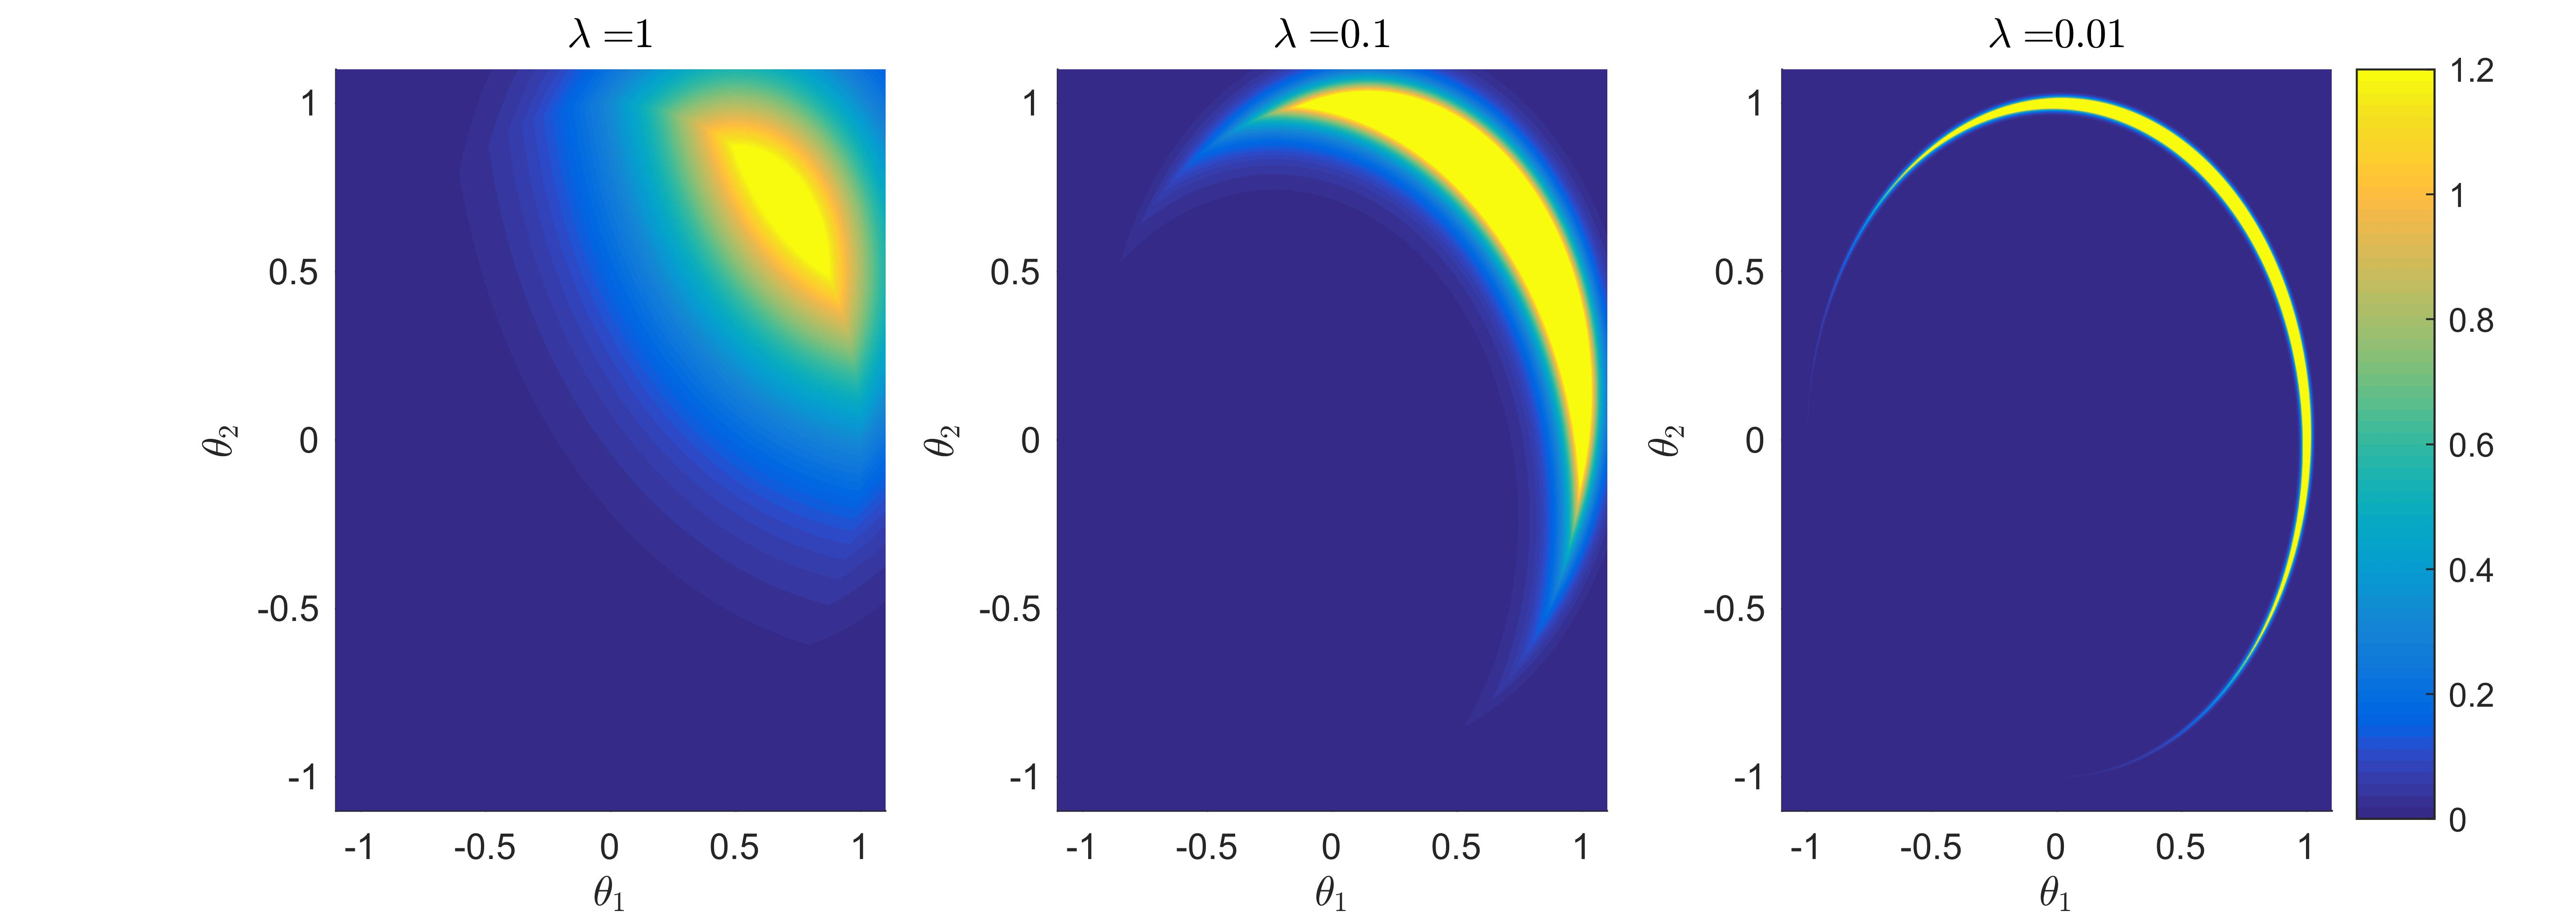
\includegraphics[width=1\textwidth]{Bivariate_Normal_Unit_Circle_Constraint}
\caption{The relaxed distribution from a von Mises--Fisher
distribution $\mbox{vMF}(
[1/\sqrt{2},1/\sqrt{2}]',1/25)$. With decreasing
$\lambda$, the relaxation is reduced and the circular
constraint becomes clear.}
\label{FIG:Bivariate_Normal_Unit_Circle_Constraint}
\end{center}
\end{figure}

\section{Theory}

In this section, we provide theoretic details, mainly on two aspects: (i)
the suitable constraints for relaxation; (ii) the error when using relaxed
model as an approximation to constrained model.

\subsection{Constrained
Space with Positive Measure } \label{SEC:Positive_measure_theory}

For constrained space with positive measure, generally, as long
as a tractable distance function exists such that $\mc D=\{\theta:
\|v(\theta)\|=0\}$, CORE is applicable.

We now focus on quantifying the difference between constrained and
relaxed densities.  Both of these densities are absolutely continuous
with respect to Lebesgue
measure on $\mathcal{R}$.  Thus, the expectation of $g$ with respect to
constrained density is

\begin{equation}
\label{EQ:Expectation_Positive_Measure_Constraint} \bb
E[g(\theta)|\theta\in\mathcal{D}] = \int_\mathcal{D}
g(\theta)\pi_\mathcal{D}(\theta)d\mu_\mathcal{R} =
\frac{\int_\mathcal{D} g(\theta)\mathcal{L}(\theta; Y)
\pi_\mathcal{R}(\theta)d\mu_\mathcal{R}(\theta)}{\int_\mathcal{D}
\mathcal{L}(\theta; Y)
\pi_\mathcal{R}(\theta)d\mu_\mathcal{R}(\theta)}.
\end{equation}

Similarly, the expected value of $g$ with respect to the relaxed density,
\begin{equation} \label{EQ:Expectation_Positive_Measure_Relaxed}
\bb E_{\tilde{\pi}_\lambda}[g(\theta)] = \int_\mathcal{R}
g(\theta)\tilde{\pi}_\lambda(\theta)d\mu_\mathcal{R} =
\frac{\int_\mathcal{R} g(\theta)\mathcal{L}(\theta; Y)
\pi_\mathcal{R}(\theta)
\exp(-\|v_{\mc
D}(\theta)\|/\lambda)d\mu_\mathcal{R}(\theta)}{\int_\mathcal{R}
\mathcal{L}(\theta; Y)\exp(-\| v_{\mc D}(\theta)\|/\lambda)
\pi_\mathcal{R}(\theta)d\mu_\mathcal{R}(\theta)}.\end{equation}

We can now consider the behavior of $E_{\tilde{\pi}_\lambda}[g]$ as $\lambda
\to 0^+.$

\begin{lemma} \label{THM:positive_measure_approximation_error} Suppose $g
\in \mathbb{L}^1(\mathcal{R},
\mathcal{L}(\theta;Y)\pi_\mathcal{R}d\mu_\mathcal{R})$.  Then,
$$\bigg|\bb E[g(\theta) \mid \theta\in\mathcal{D}] -
\bb E_{\tilde{\pi}_\lambda}[g(\theta)]   \bigg| \le
\frac{\int_{\mathcal{R}\setminus \mathcal{D}}
(C_\mathcal{R}\bb E|g(\theta)|+|g(\theta)|) \mathcal{L}(\theta; Y)
\pi_\mathcal{R}(\theta)\exp(-\|v_{\mc D}(\theta)\|/\lambda )
d\mu_\mathcal{R}(\theta)}{\big[\int_\mathcal{D} \mathcal{L}(\theta; Y)
\pi_\mathcal{R}(\theta)d\mu_\mathcal{R}(\theta)\big]^2 }$$ where
$E|g(\theta)| \propto \int_\mathcal{R} |g(\theta)|
\mathcal{L}(\theta;Y)\pi_\mathcal{R} d\mu_\mathcal{R}(\theta)$ is the
expected value of $|g(\theta)|$ with respect to the unconstrained posterior
density and $C_\mathcal{R} = \int_\mathcal{R}
\mathcal{L}(\theta;Y)\pi_\mathcal{R}(\theta)d\mu_\mathcal{R}(\theta)$ is
the normalizing constant of this unconstrained posterior density.
Furthermore, if $\|v_{\mc D}(\theta)\|$ is zero for all $\theta\in\mathcal{D}$ and
positive for $\theta\in(\mathcal{R}\setminus\mathcal{D})^o$, it follows
from the dominated convergence theorem that $$\bigg| \bb E[g(\theta)
|\theta\in\mathcal{D}] - \bb E_{\tilde{\pi}_\lambda}[g(\theta)]   \bigg|\to 0
\text{ as } \lambda \to 0^+.$$ \end{lemma}

Thus, one can obtain sufficiently accurate estimates of
$\bb E[g|\theta\in\mathcal{D}]$ by sampling from $\tilde{\pi}_\lambda$ when
$\lambda$ is sufficiently small.  From a practical standpoint, it is
desirable to understand the rate at which
$\bb E_{\tilde{\pi}_\lambda}[g(\theta)] $ converges to
$\bb E[g(\theta)\in\mathcal{D}]$. This question is addressed in the following
theorem.

\begin{theorem} \label{THM:Positive_measure_convergence_rate} Suppose $g
\in  \mathbb{L}^2(\mathcal{R},
\mathcal{L}(\theta;Y)\pi_\mathcal{R}d\mu_\mathcal{R})$,
$v_{\mc D}(\theta)= \inf_{x\in\mathcal{D}} \|\theta-x\|_2$, $\mathcal{D}$ has a piecewise smooth boundary, and that
$\mathcal{L}(\theta;Y)\pi_\mathcal{R}(\theta)$ is continuous on a
open neighborhood containing $\mathcal{D}$.  Then for $0<\lambda
\ll 1,$ $$ \bigg|\bb E[g(\theta) |\theta\in\mathcal{D}] -
\bb E_{\tilde{\pi}_\lambda}[g(\theta)]   \bigg| = O(\sqrt{\lambda}).  $$
\end{theorem} This theorem follows by applying the Cauchy-Schwartz
inequality to the term in the numerator of the bound given in Lemma
\ref{THM:positive_measure_approximation_error}.  One can attain a bound
depending on the surface area of $\mathcal{D}$ when it is bounded. The proofs of
Lemma \ref{THM:positive_measure_approximation_error} and Theorem
\ref{THM:Positive_measure_convergence_rate} are contained in Appendix
\ref{APP:Positive_Measure_Convergence_Proofs}.

These results have some important implications both analytically and
numerically.  First, in addition to point estimates,
$\bb E[\theta \mid \theta\in\mathcal{D}]$, it is possible to approximate
probabilities $P(\theta \in \mathcal{F}|\theta \in \mathcal{D})$ and higher
moments, e.g. $\bb E[\Pi_j \theta_j^{k_j} |\theta\in\mathcal{D}]$, so long as
these moments exist for the unconstrained posterior density. Second, these bounds demonstrate that the error in using the relaxed
density to approximate $\bb E[g(\theta)|\theta\in\mathcal{D}]$ is proportional
to $\sqrt{\lambda} [\int_\mathcal{D}\mathcal{L}(\theta; Y)
\pi_\mathcal{R}(\theta)d\mu_\mathcal{R}(\theta)\big]^{-2}$ although this
rate may not be optimal.  In practice, $\lambda$ may need to be very small,
particularly in the case where $0<P(\theta\in\mathcal{D})\ll 1.$ Of course,
specific details of the scaling of $\bigg|\bb E[g(\theta)
|\theta\in\mathcal{D}] - \bb E_{\tilde{\pi}_\lambda}[g(\theta)]   \bigg|$ will
depend upon $\mathcal{D}$ and $\|v_{\mc D}(\theta)\|$.

\subsection{Constrained Space with Zero Measure}
\label{SEC:Zero_measure_theory}

For the constrained space with zero measure, we review a few important concepts of
geometric measure theory which are used throughout this section.  First,
recall the definition of Hausdorff measure.  \begin{Hausdorff_def} Let
$A\subset \bb R^r$. Fix $s \le r$. Then $$\mc H^{s}(A)=
\underset{\delta\rightarrow 0}\lim \inf \bigg\{ \sum
\left[{\text{diam}(S_i)}\right]^s: {A\subseteq \cup S_i,
\text{diam}(S_i)\le \delta}, \text{diam}(S_i)=\sup_{x,y\in
S}\|x-y\|\bigg\}$$.  \end{Hausdorff_def} We denote the normalized Hausdorff
measure as $\bar{\mc H}^{s}(A) =\frac{\Gamma(\frac{1}{2})^{s}}{2^s
\Gamma(\frac{s}{2}+1)} \mc H^{s}(A)$. When $s=r$, Lebesgue and normalized
Hausdorff measures coincide  $\mu_{\mathbb{R}^m}(A)= \bar{\mc H}^{s}(A)$
\citep{evans2015measure}.  Additionally, for a subset $\mathcal{D}$, there
exists a unique, critical value $d$ such that
$$\bar{\mathcal{H}}^s(\mathcal{D}) = \begin{cases} 0, & s > d \\ \infty, &
s < d.\end{cases}$$ The critical value, $d$, is referred to as the
Hausdorff dimension of $\mathcal{D}$. We note that, when $\mathcal{D}$ is a
compact, $d$-dimensional submanifold of $\mathbb{R}^m$, it will have
Hausdorff dimension $d$ and $\bar{\mathcal{H}}^d(\mathcal{D})$ is the
$d$-dimensional surface area of $A.$

We now state the co-area formula which is used to define a regular
conditional probability on the measure zero constrained space $\mathcal{D}$
and is pivotal in all of the proofs of the theorems.
\begin{theorem}{Co-area formula \citep{diaconis2013manifold,
federer2014geometric}} Suppose $\nu:\mathbb{R}^r\to\mathbb{R}^s$
with $ s<r$ is Lipschitz and that
$g\in\mathbb{L}^1(\mathbb{R}^r,\mu_{\mathbb{R}^r}).$ Assume
$J[\nu(\theta)]>0$, then \begin{equation} \int_{\mathbb{R}^r}
g(\theta)J[\nu(\theta)]d\mu_{\mathbb{R}^r}( \theta)=
\int_{\mathbb{R}^s} \bigg( \int_{\nu^{-1}(y)}g(\theta)
d\bar{\mathcal{H}}^{r-s}(\theta)\bigg)d\mu_{\mathbb{R}^s}(y),
\end{equation} \end{theorem} The behavior of the pre-images
$\nu^{-1}(y)$ in the co-area formula are important for the
convergence results presented later in this section.  As such, we assume that $\mathcal{D}$ can be defined implicitly as the
solution set to a system of $s$ equations,  $\{\nu_j(\theta)=0\}_{j=1}^s$,
where \begin{itemize} \item[(a)] $\nu_j:\mathcal{R}\to\mathbb{R}$ is
Lipschitz continuous, \item[(b)] $v_j(\theta)=0$ only for
$\theta\in\mathcal{D}$, \item[(c)] for $j=1,\dots, s$, the
pre-image
$v_j^{(-1)}(x)$ is a co-dimension 1 sub-manifold of $\mathcal{R}$
for $\mu_\mathbb{R}$-a.e. $x$ in the range of $v_j$, \item[(d)]
$v_j^{(-1)}(0)$ and $v_k^{(-1)}(0)$ intersect transversally for
$1\le j<k\le s.$ \end{itemize}

We refer to the functions
$v_1,\dots,v_s$ as constraint functions. In this case, if we
let $\nu:\mathcal{R}\to \mathbb{R}^s$ be the vector-valued function
$\nu(\theta) = [\nu_1(\theta),\dots,\nu_s(\theta)]^T$, then
$\mathcal{D} = \ker(v)$ is a co-dimension $s$ submanifold of
$\mathcal{R}$ for $\mu_{\mathbb{R}^s}$-a.e. $x$ the range of $v.$
Recall, the ambient space, $\mathcal{R}$, is $r-$dimensional.
Therefore, it follows that $\mathcal{D}$ is a $(r-s)-$dimensional
submanifold of $\mathcal{R}$, and it is natural to discuss the
$(r-s)$-dimensional surface area of $\mathcal{D}.$

Property (a), guarantees that $\nu$ is itself Lipschitz.  The remaining
properties (b)-(d) are constructed so that $\nu^{(-1)}(x)$ for
$x\in\mathbb{R}^s$ is also a submanifold which is close to
$\mathcal{D}=\nu^{(-1)}(0)$ when $x$ is near zero.  In particular, the
assumption of transversality ensures that $\nu^{(-1)}(x)$ with also be
$r-s$ dimensional for $x$ sufficiently close to 0, \leo{defined by the
set $\mc X$}.


The existence and uniqueness of the constraints must be addressed.  In the
case where $\mathcal{D}$ is specified by a collection of equality
constraints -- such as the probability simplex or the Stiefel manifold for
example--  it is not difficult to find a suitable set of constraint
functions. Table \ref{TABLE:Equality_constraints_examples} contains a
number of examples of common constrained spaces and appropriate choices of
constraint functions.  \renewcommand{\arraystretch}{1.5} \begin{table}[h!]
\begin{center} \begin{tabular}{| c | m{4 cm} | c | c | m{6cm} |}
\hline $\mathcal{R}$                           &
$\mathcal{D}$                                  &
$\dim(\mc R)$                                  &
$\dim( \mc D)$                                 & Constraint functions                                  \\ \hline $[0,1]^r$ &
Probability simplex, $\Delta^{r-1}$            & $r$                            & $r-1$ & $v(\theta)
= \sum(\theta) -1$                                                                                     \\ \hline $\mathbb{R}^r$ & Line,
span$\{\vec{u}\}$ \newline $\vec{u}\ne\vec{0}$ & $r$                            & $1$
&
$\nu_j(\vec{\theta}) = \vec{\theta}\,^T\vec{b}_j$ \newline
$\{\vec{b}_1,\dots,\vec{b}_{r-1}\}$ a basis for
span$\{\vec{u}\}^\perp$                                                                                \\ \hline $[-1,1]^r$ & Unit
sphere, $\mathbb{S}^{r-1}$                     & $r$                            & $r-1$ & $v(\theta) =
(\|\theta\|^2 -1)$                                                                                     \\ \hline $[-1,1]^{n\times
k}$                                            & Stiefel manifold, $\mc V(n,k)$ & $nk$  & $nk -
\frac{1}{2}k(k+1)$                             & $v_{i,j}(\theta) = (
\vec{\theta}_i'\vec{\theta}_j- \delta_{i,j})$ \newline
$1\le i \le j \le k$ and $\delta_{i,j} = \mathbbm{1}_{i=j}$
\\ \hline\end{tabular} \end{center} \caption{Table of
constraints for some commonly used constrained spaces.}
\label{TABLE:Equality_constraints_examples} \end{table}


With regards to uniqueness, we note that the constraints cannot be unique
in any case.  For example, rescaling in each $v_j(\theta)$ will also satisfy (a)-(d). Naturally, an optimal choice will depend largely on the properties of the constrained distribution that one wishes to estimate making the choice of
$\{\nu_j\}_{j=1}^s$ context dependent.

Under the given construction of the constrained space, we can now specify the regular conditional probability of $\theta$, given $\theta \in
\mathcal{D}.$

\begin{theorem}\citep{diaconis2013manifold}
\label{THM:RCP_construction} Assume that $J(v(\theta)) > 0$ and
that for each $z\in\mathbb{R}^s$ there is a finite non-negative
$p_z$ such that,  $$m^{p_z}(z) = \int_{v^{-1}(z)}
\frac{\mathcal{L}(\theta; Y) \pi_\mathcal{R}(\theta)}
{J(v(\theta))}
d\bar{\mathcal{H}}^{p_z}(\theta)
\in (0,\infty).$$

Then, for any Borel subset $F$ of
$\mathcal{R}$, it follows that $$P(F \mid v(\theta) = z) = \begin{cases}
\frac{1}{m^{p_z}(z)} \int_{F} \frac{\mathcal{L}(\theta; Y)
\pi_\mathcal{R}(\theta)
\mathbbm{1}_{v(\theta)=z}}{J(v(\theta))}
d\bar{\mathcal{H}}^{p_z}(\theta)
& m^p(z)\in (0,\infty) \\ \delta (F) & m^p(z) \in \{0,\infty\}
\end{cases}$$
is a valid regular conditional probability for
$\theta\in\mathcal{D}.$ Here, $\delta (F)=1$ if $0\in F$ and $0$ otherwise.
\end{theorem}

\leo{
By construction, $\{\theta:v(\theta)=z\}$ is a $(r-s)$ dimensional
submanifold of $\mathcal{R}$ for $\mu_{\mathbb{R}^s}$-a.e. $z$ in $\mc X$,
the suitable range
of $v$. As such, it follows that one should take $p_z=r-s$. It is possible that
$m^p(z)\in\{0,\infty\}$ for some $z\not\in \mc X$; however, they are excluded during our construction. Most importantly, $0\in \mc X$,
therefore,} Theorem~\ref{THM:RCP_construction} allows us to define

\begin{equation} \label{EQ:Constrained_rcp}
\pi_\mathcal{D}(\theta|\theta\in\mathcal{D},Y) = \frac{1}{m^{r-s}({0})}
\frac{\mathcal{L}(\theta; Y) \pi_\mathcal{R}(\theta)
\mathbbm{1}_{v(\theta)={0}}}{J(v(\theta))} \end{equation} as the
constrained posterior density.

As a result, we
can define the conditional expectation of $g(\theta)$ given $\theta \in
\mathcal{D}$ as
$$\bb E[g(\theta) | \theta\in\mathcal{D}] = \bb E[g(\theta) |
\nu(\theta) =0\,] = \int_\mathcal{R} g(\theta) \pi_\mathcal{D}(\theta)
d\bar{\mathcal{H}}^{r-s}(\theta).$$

The expected value of
$g(\theta)$ with respect to the relaxed density, denote
$\bb E_{\tilde{\Pi}}[g(\theta)] $, is

$$\bb E_{\tilde{\Pi}}[g(\theta)] = \frac{1}{m_\lambda}
\int_\mathcal{R} g(\theta) \pi_\mathcal{R}(\theta)
\mathcal{L}(\theta;Y)\exp\bigg(-\frac{1}{\lambda}\|\nu (\theta)\|_1\bigg)
d\mu_\mathcal{R}(\theta) $$
with $m_\lambda =
\int_\mathcal{R}  \pi_\mathcal{R}(\theta)
\mathcal{L}(\theta;Y)\exp(-{\lambda^{-1}}\|\nu (\theta)\|_1)
d\mu_\mathcal{R}(\theta).$
The primary results of the section are the following statements regarding
the use of $\bb E_{\tilde{\Pi}}[g]$ to estimate $\bb E[g|\theta\in\mathcal{D}]$.

\begin{theorem} \label{THM:Relaxed_Expectation_Convergence_Measure_Zero}
Let $m:\mathbb{R}^s\to \mathbb{R}$ and $G:\mathbb{R}^s\to
\mathbb{R}$ be defined as follows \begin{align*} m(x) & =
\int_{\nu^{-1}(x)} \frac{\pi_\mathcal{R}(\theta)
\mathcal{L}(\theta;Y)}{J(\nu(\theta))}
d\mathcal{R}^{r-s}(\theta) \\ G(x) &= \int_{\nu^{-1}(x)}
g(\theta)\frac{\pi_\mathcal{R}(\theta)
\mathcal{L}(\theta;Y)}{J(\nu(\theta))} d\mathcal{R}^{r-s}(\theta).
\end{align*} Suppose that both $m$ and $G$ are continuous on an open
interval containing the origin and that \\
$g\in\mathbb{L}^1(\mathcal{R},\pi_R\mathcal{L}(\theta;Y)d\mu_\mathcal{R})$.
Then, $$\bigg|\bb E_{\tilde{\Pi}}[g] - \bb E[g|\theta \in \mathcal{D}]\bigg| \to 0
\text{ as } \lambda\to 0^+.$$ \end{theorem}

\begin{corollary} In addition to the assumptions of Theorem
\ref{THM:Relaxed_Expectation_Convergence_Measure_Zero}, suppose
that both $m$ and $G$ are differentiable at $0$. Then
$$\bigg|\bb E_{\tilde{\Pi}}[g] - \bb E[g|\theta \in \mathcal{D}] \bigg| =
O\bigg(\frac{\lambda}{|\log \lambda|^s}\bigg)$$ as $\lambda \to
0^+.$ \end{corollary}

Like the results from Section 3.1, the convergence rates are sub-linear. Unlike the positive measure case, the convergence rates are dimension dependent. We assess the approximation error with different $\lambda$ in the von Mises--Fisher distribution as described above. The result is provided in the appendix. 


\section{Posterior Computation}

Compared to constrained density in  space $\mc D$, relaxed density is supported in $\mc R$ and can be directly
sampled via off--the--shelf tools such as slice
sampling, adaptive Metropolis-Hastings and Hamiltonian Monte Carlo (HMC).
In this section, we focus on HMC for its easiness to use and good
performance in block updating of parameters.

\subsection{Hamiltonian Monte Carlo under Constraint Relaxation}

We provide a brief overview of HMC for continuous $\theta^*$ under
constraint relaxation. Discrete extension is possible via recent work of
\cite{nishimura2017discontinuous}.

In order to sample $\theta$, HMC introduces an auxiliary momentum variable $p
\sim \No(0, \mass)$. The covariance matrix $\mass$ is referred to as a
\textit{mass matrix} and is typically chosen to be the identity or adapted
to approximate the inverse covariance of $\theta$. HMC then sample from the
joint target density $\pi(\theta, p) = \pi(\theta) \pi(p) \propto \exp (- H(\theta, p))$
where, in the case of the posterior under relaxation,


\begin{equation} \begin{aligned}
H(\theta, p) & = U(\theta)+K(p), \\ \text{where } &
U(\theta) = -\log\pi(\theta),    \\ & K(p) = \frac{p'\mass^{-1} p}{2}.
\end{aligned}
\end{equation}
with $\pi(\theta)$ is the unnormalized density in \eqref{EQ:relaxedDensityPosMeasure} or \eqref{EQ:relaxedDensityZeroMeasure}.

From the current state $(\theta^{(0)},p^{(0)})$, HMC generates a proposal for
Metropolis-Hastings algorithm by simulating Hamiltonian dynamics, which is
defined by a differential equation:

\begin{equation} \begin{aligned} \label{hamiltonian} \frac{\partial \theta
^{(t)}}{\partial t} & =\frac{\partial H(\theta, p)}{\partial p} =
\mass^{-1}p,                                                      \\ \frac{\partial p^{(t)}}{\partial t}&
=-\frac{\partial H(\theta, p)}{\partial \theta} = -\frac{\partial
U(\theta)}{\partial \theta}.\end{aligned} \end{equation}

The exact solution to \eqref{hamiltonian} is typically intractable but a
valid Metropolis proposal can be generated by numerically approximating
\eqref{hamiltonian} with a reversible and volume-preserving  integrator
\citep{neal2011mcmc}. The standard choice is the \textit{leapfrog}
integrator which approximates the evolution $(\theta^{(t)},p^{(t)}) \to (\theta^{(t +
\dt)},p^{(t + \dt)})$ through the following update equations:

\begin{equation} \begin{aligned} \label{leap-frog}
p \leftarrow p -
\frac{\dt}{2} \frac{\partial U}{\partial  \theta },\quad \theta \leftarrow  \theta
+ \dt \mass^{-1}p,\quad p \leftarrow p -  \frac{\dt}{2}
\frac{\partial U}{\partial  \theta }\end{aligned} \end{equation} Taking
$L$ leapfrog steps from the current state $(\theta^{(0)},p^{(0)})$
generates a proposal $(\theta^{*},p^{*}) \approx (\theta^{(L \dt)},p^{(L
\dt)})$, which is accepted with the probability $$1\wedge \exp
\left( - H(\theta^{*},p^{*}) + H(\theta^{(0)},p^{(0)}))\right)$$

We refer to this algorithm as CORE-HMC.

\subsection{Computing Efficiency in CORE-HMC}

Since CORE expands the support from $\mc D$ to $\mc R$, it is useful to
study the effect of space expansion on the computing efficiency of HMC. In this
subsection, we provide some quantification.

In understanding the computational efficiency of HMC, it is useful to
consider the number of leapfrog steps to be a function of $\dt$ and set $L
= \lfloor \tau / \dt \rfloor$ for a fixed integration time $\tau > 0$. In
this case, the mixing rate of HMC is completely determined by $\tau$ in the
limit $\dt \to 0$ \citep{betancourt17}. In practice, while a smaller
stepsize $\dt$ leads to a more accurate numerical approximation of
Hamiltonian dynamics and hence a higher acceptance rate, it takes a larger
number of leapfrog steps and gradient evaluations to achieve good mixing.
For an optimal computational efficiency of HMC, therefore, the stepsize
$\dt$ should be chosen only as small as needed to achieve a reasonable
acceptance rate \citep{beskos13, betancourt14}. A critical factor in
determining a reasonable stepsize is the \textit{stability limit} of the
leapfrog integrator \citep{neal2011mcmc}. When $\dt$ exceeds this limit,
the approximation becomes unstable and the acceptance rate drops
dramatically. Below the stability limit, the acceptance rate $a(\dt)$ of
HMC increases to 1 quite rapidly as $\dt \to 0$ and in fact satisfies
$a(\dt) = 1 - \mc O(\dt^4)$ \citep{beskos13}.

For simplicity, the following discussions assume the mass matrix $\mass$ is
taken to be the identity, and $\mc D= \cap_{j=1}^s\{\theta :v_j(\theta)=0 \}$.
We denote $\mc D_j= \{\theta :v_j(\theta)=0 \}$ and consider a directional
relaxation, which is equivalent to replacing a single $\lambda$ with several
$\lambda_j$'s in the relaxation part, i.e. $\exp(-\sum_j{\|v_j(\theta^*)\|}{\lambda_j^{-1}})$. There are generally two factors limiting the efficiency of HMC:
(i) the width of support in constrained space; (ii) the largest eigenvalue of the Hessian matrix.
For the former, using $\mc Q$ to denote a support, the width of support is related to the shortest
distance to the boundary $\eta (\theta; {\mc Q})= \inf_{\theta'\not\in \mc
Q}\|\theta'-\theta\|$. If $\eta (\theta; {\mc Q}) \approx 0$ for all $\theta\in \mc Q$,
the proposal would likely be rejected using a large leap-frog step size. In such case,
it is useful to utilize CORE to expand support and
increase $\eta (\theta; {\mc Q})$ for better computing efficiency. For the eigenvalue,
let $\hess_U(\theta)$ denote the hessian matrix of
$U(\theta) = - \log \pi(\theta)$.
The linear stability analysis and
empirical evidences suggest that, for stable approximation of Hamiltonian
dynamics by the leapfrog integrator in $\bb R^p$, the condition $\dt <
2\xi_1(\theta)^{-1/2}$ must hold on most regions of the parameter space
\citep{hairer06}, with $\xi_1(\theta)$ the largest
eigenvalue of $\hess_U(\theta)$. The hessian is

\begin{equation} \label{eq:hessian_extrinsic}
\hess_U(\theta) = -\hess_{\log
(\mathcal L(\theta;y) \pi_{\mc R}(\theta))
}(\theta)+\sum_j \lambda_j^{-1} \hess {\|v_j(\theta)\|}
\mathbbm{1}_{\theta\not\in \mc D_j}. \end{equation}
Note the second term is zero unless $\theta$ is outside of $\mc D_k$. As $\lambda^{-1}_j$ in the
second term often dominates the eigenvalue in the first term, hence the effective eigenvalue often is
proportional to $ \underset{j: \theta \not\in \mc D_j}{\min}\lambda_j^{1/2}$.

Lastly, one may want to use CORE for approximate estimation under constrained
model, while maintaining some computing efficiency.
For this purpose, we now provide a practical guide on choosing $\lambda_j$.  For $\mc
D_j$'s with very small distance to support boundary $\eta(\theta;\mc D_j)\approx 0$, one should use moderate $\lambda_j$
to increase support width;  for $\mc D_j$'s
without this issue, one should use very small $\lambda_j\approx 0$ to keep $\theta\in\mc D_j$, so that it has almost no influence on the hessian eigenvalue.
The high rejection of HMC near the boundary of $\mc D_j$ can be avoided with random step size $\epsilon$ at each iteration, which is recommended for HMC in general \citep{livingstone2016geometric}. We evaluate the computing efficiency with different $\lambda$ in sampling the von Mises--Fisher distribution. The result is provided in the appendix.

\section{Simulated Examples}

The simple computation of CORE frees up the modeling flexibility. We now illustrate more utility of the method via simulated examples.

\textbf{Example: Sphere $t$ Distribution}

We now derive a new distribution on a $(p-1)$-sphere $\mc
D=\{\theta\in
\bb R^p:\|\theta\|_2 =1\}$. Recall that von
Mises--Fisher distribution \citep{khatri1977mises} is the result of
constraining a multivariate Gaussian $\theta \sim \No(F,I\sigma^2)$ with
$F\in \mc D$ 

$$
\pi_{\mc D}(\theta) \propto
\exp(-\frac{\|F-\theta\|^2}{2\sigma^2})
\mathbbm{1}_{\theta'\theta=1} \\
\propto
\exp(\frac{F'}{\sigma^2}\theta)
\mathbbm{1}_{\theta'\theta=1}.
$$
Although the final form
appears more
like an exponential, the behavior of von
Mises--Fisher
on sphere can be largely explained by its unconstrained parent Gaussian.
In the Gaussian $\pi_{\mc
R}(\theta)$, $\theta$ is symmetrically distributed around $F$, with density
decaying exponentially as $\| \theta-F\|^2$ increases with rate
$({2\sigma^2})^{-1}$; as the constrained
density $\pi_{\mc D}(\theta)$ is proportional $\pi_{\mc R}(\theta)$, it concentrates
similarly.

This naturally suggests we could use another distribution to induce different behavior on the sphere; then one could use CORE to generate approximate sample. We start from a
multivariate $t$-distribution $\pi_{\mc
R}(\theta)$, $t_m(F,I\sigma^2)$ with $m$ degrees of freedom,
mean $F\in \mc D$ and variance $I\sigma^2$, using \eqref{EQ:Constrained_rcp} to generate a density
\be
\pi_{\mc
D}(\theta)
\propto &
(1+\frac{\|F-\theta\|^2}{m\sigma^2})^{-\frac{(m+p)}{2}}\mathbbm{1}_{\theta'\theta=1}\\
\propto &
(1-\frac{F'\theta}{1+m\sigma^2/2})^{-\frac{(m+p)}{2}}\mathbbm{1}_{\theta'\theta=1}
\ee
As in the $t$-distribution, the density decays polynomially as $\|F-\theta\|^2$ increases, as opposed to the exponential decay in Gaussian. We refer to this new distribution as sphere $t$-distribution.

CORE allows us to easily obtain approximate sample via relaxation function $\exp(- \lambda^{-1}\|\theta'\theta-1\|)$. Figure~\ref{sphere_examples} shows that the sphere t-distribution with $m=3$ exhibits much less concentration than von Mises--Fisher on the sphere,. This can be useful for robust modeling when there could be `outlier' on the sphere.
\begin{figure}[H]
\begin{subfigure}[b]{0.45\textwidth}
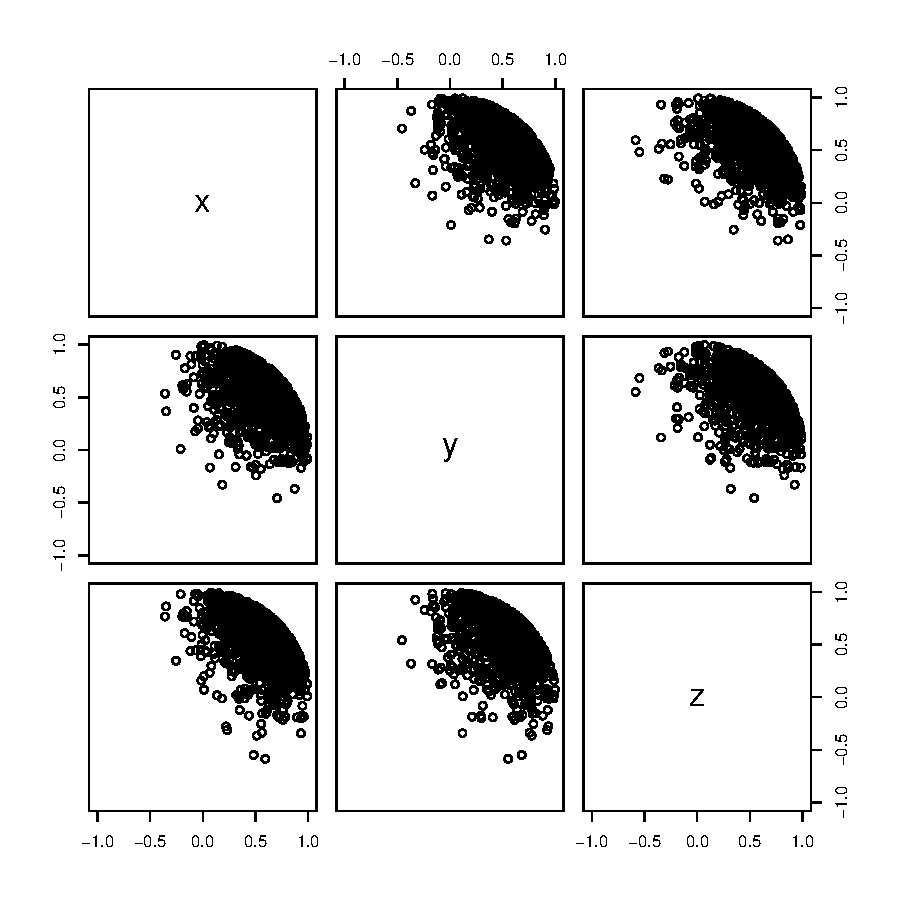
\includegraphics[width=1\textwidth]{sphere_vmf.pdf}
\caption{von Mises--Fisher distribution.}
\end{subfigure}
\begin{subfigure}[b]{0.45\textwidth}
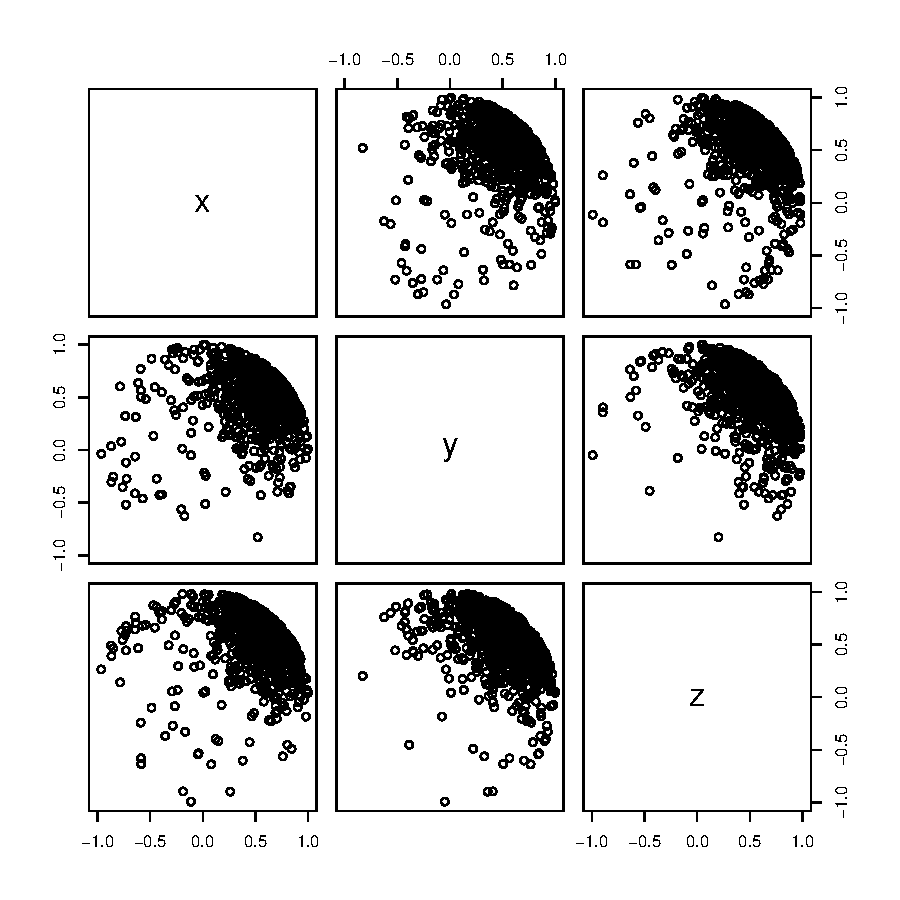
\includegraphics[width=1\textwidth]{sphere_t}
\caption{Sphere $t$-distribution with $m=3$.}
\end{subfigure}
\caption{Sectional view of random samples from constrained distributions on a unit sphere inside $\bb R^3$. The distributions are derived through conditioning on $\theta'\theta=1$ based on unconstrained densities of (a) $\No( F, \diag\{0.1\})$, (b) $t_3(F,\diag\{0.1\} )$, where $F=[1/\sqrt{3},1/\sqrt{3},1/\sqrt{3}]'$. The samples are generated via CORE-HMC with $\lambda=10^{-3}$.
}
\label{sphere_examples}
\end{figure}

\textbf{Example: Ordered Dirichlet Distribution}

We derive an ordered Dirichlet distribution. We build it upon the canonical Dirichlet distribution $\mbox{Dir}(\alpha)$ with $
\pi_{\mc D}(\theta) \propto \prod_{j=1}^J \theta_j^{\alpha-1} \1_{\sum_{j=1}^J \theta_j=1}$ and further impose order constraint, $1> \theta_1 \ge \ldots \ge \theta_J > 0$, yielding


\begin{equation}
\begin{aligned}
\label{ordered_dp_prior}
\pi_{\mc D}(\theta) \propto \prod_{j=1}^J \theta_j^{\alpha-1} \cdot \1_{\sum_{j=1}^J \theta_j=1} \cdot  \prod_{j=1}^{J-1}\1_{\theta_j \ge \theta_{j+1}}.
\end{aligned}
\end{equation}

As commonly used in mixture model, canonical Dirichlet prior has its index $j$ exchangeable. Since its permutation does not change the likelihood, label-switching problem often occurs (reviewed in \cite{jasra2005markov}). Naturally, order constraint in $\theta$ can alleviate this problem, especially in preventing the switch between large $\theta_j$ and small $\theta_{j'}$.

To illustrate, we consider a hierarchical normal distribution with a common variance but the mean from a mixture, for data $y_i\in \bb R^2$ indexed by $i=1,\ldots,n$:

\begin{equation*}
\begin{aligned}
y_i   & \stackrel{indep}{\sim} \No(\mu_i,\Sigma),\qquad
\mu_i & \stackrel{iid}{\sim} G,\qquad
G(.)  & = \sum_{j=1}^{J} \theta_j \delta_{\mu_j}(.),
\end{aligned}
\end{equation*}

We generate $n=100$ samples from $3$ components with $\{\theta_1,\theta_2,\theta_3\}=\{0.6,0.3,0.1\}$, $\{\mu_1,\mu_2,\mu_3\} = \{[1,5], [3,3], [3,5]\}$ and $\Sigma = I_2$. We assign weakly informative priors $\No(0,10 I_2)$ for each $\mu_j$ and inverse--Gamma prior for the diagonal element in $\Sigma=\diag(\sigma_1^2,\sigma_2^2)$ with $\sigma^2_1, \sigma^2_2\sim \mbox{IG}(2,1)$.  Figure~\ref{dirichlet}(a) shows the contour of posterior density of $\mu$. The small component sample size leads to large overlap among the posterior.


\begin{figure}[H]
\begin{center}
\begin{subfigure}[b]{0.6\textwidth}
\centering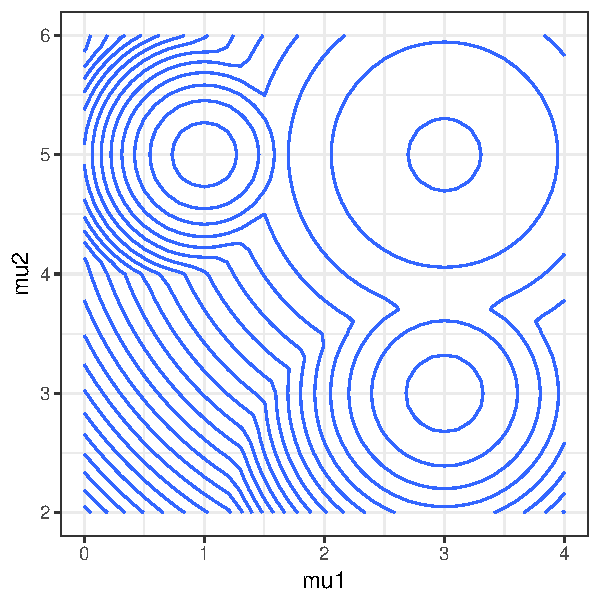
\includegraphics[width=0.5\textwidth]{fmm_mu_contour.pdf}
\caption{\small Posterior density of the component means $\{\mu_j\}_{j=1}^3$.}
\end{subfigure}
\end{center}
\centering
\begin{subfigure}[b]{0.32\textwidth}
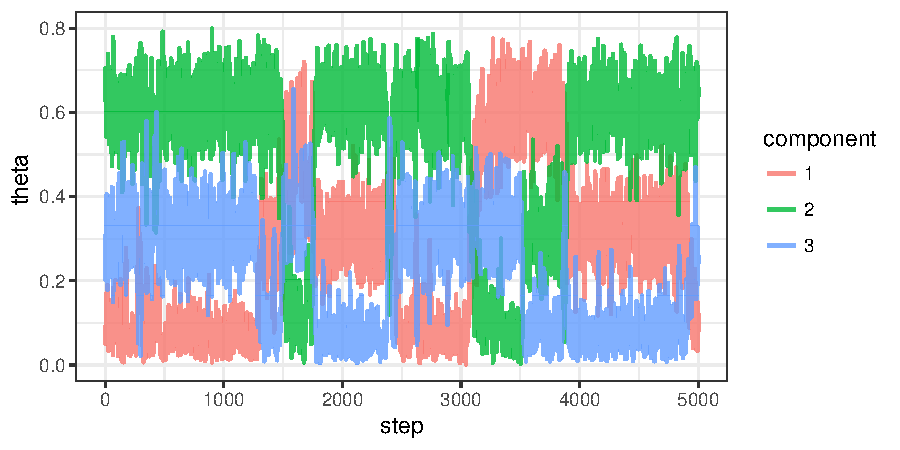
\includegraphics[width=1\textwidth]{fmm_w_gibbs.pdf}
\caption{\small  Gibbs sampling of unordered Dirichlet}
\end{subfigure}
\begin{subfigure}[b]{0.32\textwidth}
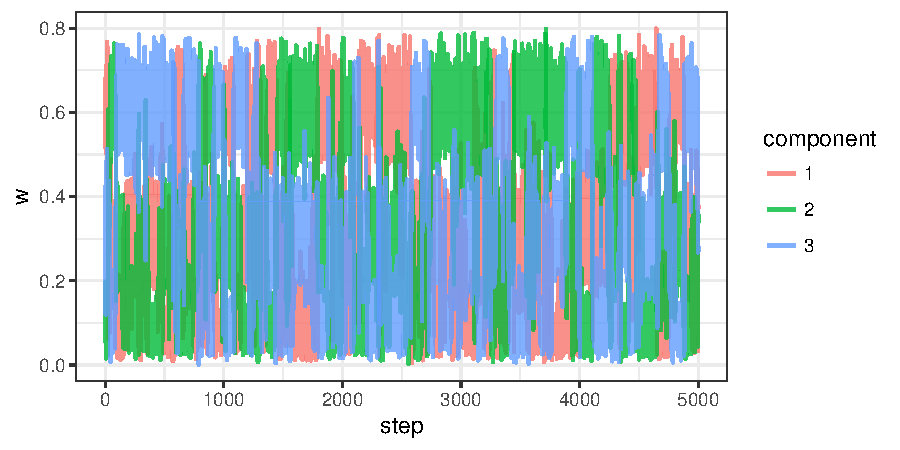
\includegraphics[width=1\textwidth]{fmm_w_hmc_unordered.pdf}
\caption{\small  HMC sampling of unordered Dirichlet}
\end{subfigure}
\begin{subfigure}[b]{0.32\textwidth}
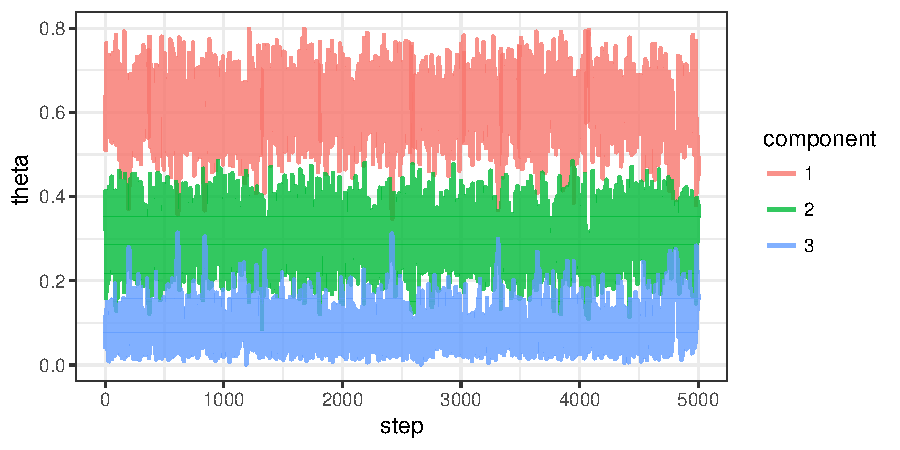
\includegraphics[width=1\textwidth]{fmm_w_hmc.pdf}
\caption{\small  HMC sampling of ordered Dirichlet}
\end{subfigure}
\caption{Contour of the posterior density of component means and traceplot of the posterior sample for the component weights $w$, in a 3-component normal mixture model. Panel (a) shows that there is significant overlap among component means $\{\mu_j\}_{j=1}^3$. Without ordering in $\theta$, its traceplot shows label-switching issue in both Gibbs (b) and HMC  (c) sampling of Dirichlet distribution. The ordered Dirichlet distribution has significantly less label-switching issue (d), where we utilize CORE to obtain approximate posterior sample.}
\label{dirichlet}
\end{figure}


The ordering disrupts the traditional Gibbs sampling \citep{ishwaran2001gibbs}, however, one could still obtain approximate posterior using CORE. We use $
\exp ( -  \lambda_1^{-1} \| \sum_{j=1}^J  \theta_{j} - 1) \|)
\prod_{j=1}^{J-1} \exp [ -  \lambda_2^{-1}  \max( \theta_{j+1} -
\theta_j,0)]  $ to relax the constraints. We use $\lambda_1 =
10^{-3}$ on simplex constraint to allow efficient sampling and
$\lambda_2 = 10^{-6}$ to induce almost no relaxation on the
ordering. The posterior estimates of $\theta$ in CORE are
close to the true values and indistinguishable from the other
methods, except for a very small relaxation $\sum_{j=1}^J\theta_j-1$ at
posterior mean $0.001$ ($(-0.001,0.003)$ for $95\%$ credible interval).

We compare the traceplots of ordered Dirichlet and unordered Dirichlet.
Without the order constraint, significant label-switching occur in both
Gibbs and HMC (traceplots in Figure~\ref{dirichlet}(b,c)), whereas ordered
Dirichlet has almost no label-switching( Figure~\ref{dirichlet}(d)).

\section{Application: Sparse Latent Factor Model in a Population of Brain Networks}

We apply CORE in a real data application of analyzing a population of brain
networks. The brain connectivity structures are obtained in the data set
KKI-42 \citep{landman2011multi}, which consists of $n=21$ healthy subjects
without any history of neurological disease. For each subject, we take the
first scan out of the scan-rescan data as the input data, and reserve the
second scan for model validation later. Each observation is a $V\times V$
symmetric network, recorded as an adjacency matrix $A_i$ for
$i=1,\ldots,n$. The regions are constructed via the
\cite{desikan2006automated} atlas, for a total of V = 68 nodes (brain regions).  For the $i$th matrix
$A_i$, $A_{i,k,l} \in \{0,1\}$ is the element on the $k$th row and $l$th
column of $A_i$, with $A_{(i,k,l)}=1$ indicating there is an connection
between $k$th and $l$th region, $A_{(i,k,l)}=0$ if there is no connection.
The matrix is symmetric with the diagonal records empty $A_{(i,k,k)}$ for
all $i$ and $k$.

One interest in neuroscience is to quantify the variation of
brain networks and identify the brain regions contributing to difference.
Extending latent factor model to multiple matrices, one appealing approach is
to have the networks share a common factor matrix but let the loadings
vary across subjects.

\begin{equation*} \begin{aligned}
& A_{(i,k,l)} \sim \text{Bern}( \frac{1}{1+ \exp(-\psi_{(i,k,l)}-
z_{(k,l)})})                                                             \\ & \psi_{(i,k,l)} = \sum_{r=1}^{d}  v_{(i,r)} u_{(k,r)}
u_{(l,r)}                                                                \\
& z_{(k,l)} \sim \No(0,\sigma^2_z),\quad  \sigma^2_z\sim \text{IG}(2,1) \\
& v_{(i,r)} \sim \No(0,\sigma^2_{v,(r)}), \quad
\sigma^2_{v,(r)} \sim \text{IG}(2,1)
\end{aligned} \end{equation*}
for
$k>l$, $k=2,\ldots, V$, $i=1,\ldots,n$;  we choose weakly informative prior inverse
Gamma $\text{IG}(2,1)$, as appropriate for the scale parameters $\sigma^2_.$ under the logistic
link; $Z=\{z_{(k,l)}\}_{k=1,\ldots,V;l=1,\ldots,V}$ is a symmetric unstructured
matrix that serves as the latent mean; $\{ v_{(i,r)}\}_{r=1,\ldots,d}$ is
the loading for the $i$th network, with each $v_{(i,r)}>0$; $U=\{ u_{(k,r)}\}_{ k=1,\ldots,V;r=1,\ldots,d}$ is the $V\times d$ shared factor matrix.

To help convergence, it is common to let the factor matrix $U$ on a Stiefel manifold $\mc V(n,d)=\{U: U'U=I_d\}$, so that free rotation or rescaling of $U$ is less likely to  occur \citep{hoff2016equivariant}. Obviously, slightly relaxing this constraint via CORE can still retain this convergence property, at this time, much more flexible priors can be assigned for $U$.


%  Using $r$ to index
% $1,\ldots,d$, each frame $U_r$ represents a $(n-1)$-hypersphere. Applying
% shrinkage forces some of its sub-coordinates to be close to $0$, which is
% reducing each $U_r$ onto a lower-dimensional hypersphere.  Although
% previous work was done using sparse PCA \citep{zou2006sparse} for
% continuous outcome,  little work has been done in a probabilistic model for
% binary matrices.

We now consider apply a shrinkage prior near the Stiefel manifold, in order to  identify the important nodes. We use the Dirichlet-Laplace prior \citep{bhattacharya2015dirichlet}:

\begin{equation*} \begin{aligned}
& u_{(k,r)}= \eta_{(k,r)}\kappa_{(k,r)}\sigma_{u} \\
&
\eta_{(k,r)}\sim \text{Lap}(0,1), \quad \{\kappa_{(1,r)}\ldots
\kappa_{(V,r)}\} \sim \text{Dir}(\alpha), \quad \sigma^2_{u}\sim
\text{IG}(2,1)                                     \\\end{aligned} \end{equation*}
for $k=1,\ldots, V$,  $\text{Lap}(0,1)$ denotes the
Laplace distribution centered at $0$ with scale $1$. To induce sparsity in each Dirichlet, we use $\alpha=0.1$ as
suggested by \cite{bhattacharya2015dirichlet}. We replace the constraint by relaxation function $\exp( - \lambda^{-1} \|U'U-I\|)$, with $\lambda=10^{-3}$.

For comparison, we test with the specified model against two baseline
models:
one without
shrinkage prior; one without the shrinkage prior and
close-to orthonormality constraint. We use simple $u_{(k,r)}\sim\No(0,1)$ in those two models. We run all
models for $10,000$ iterations and discard the first $5,000$ iteration as
burn-in.  For each iteration, we run $300$ leap-frog steps. For efficient
computing, we truncated $d=20$.

Figure~\ref{network_model_basis}(a) plots the top $6$ factors $U_r$ estimated near the Stiefel manifold, without and with shrinkage prior. Under the shrinkage prior, sparsity starts to show as early as the third factor $U_3$; the second factor $U_2$ shows a clear partition of first $34$ and latter $34$ nodes, which correspond to the two hemispheres of the brain. Accordingly, in the estimated loadings $v_{(i,r) }$ (Figure~\ref{network_model_basis}(b)), model under shrinkage prior detects more variability in the subject-specific loadings (represented by each line), especially over the second factor.



For the model with a completely unconstrained $U$, the factors and loadings fail to converge. And the loadings have a much slower drop to $0$, compared to the two models with $U$ near the Stiefel manifold. This
indicates that near-orthogonal factors are more efficient representation of
the span.

\begin{figure}[H] \centering
\begin{subfigure}[b]{1\textwidth}
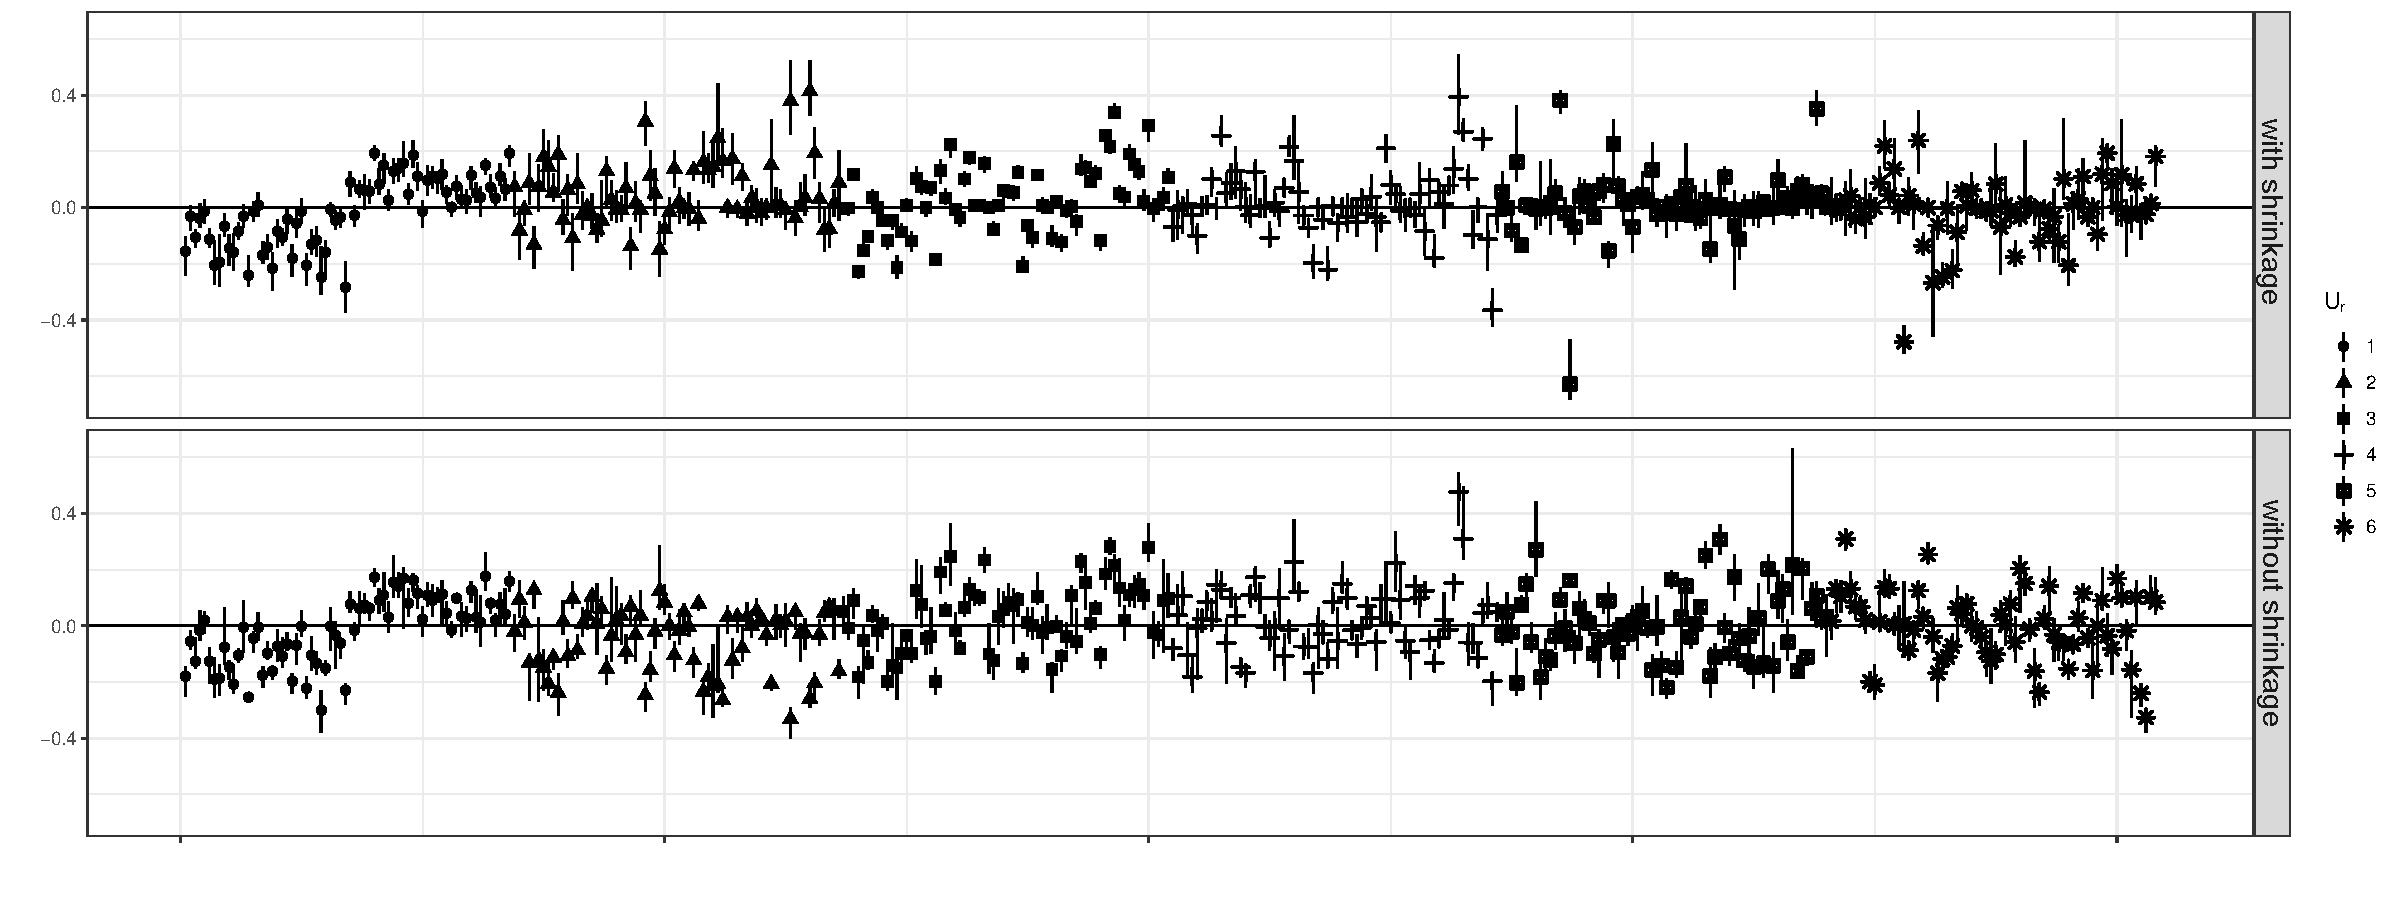
\includegraphics[width=1\textwidth]{network_factor.pdf}
\caption{Posterior mean and pointwise $95\%$ credible interval of
the factors $U_1,\ldots, U_6$ in the two constrained
models. } \end{subfigure}
\begin{subfigure}[b]{0.8\textwidth}
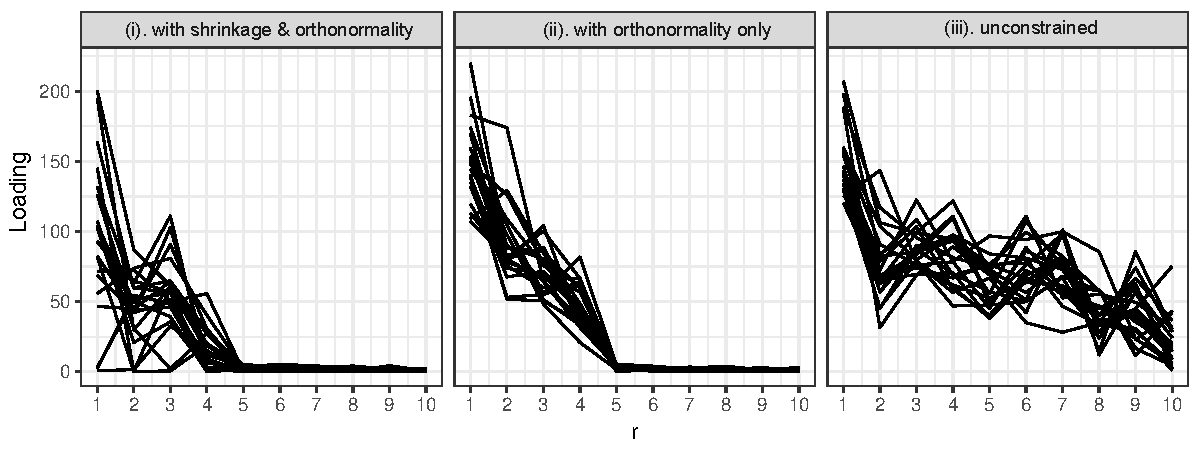
\includegraphics[width=1\textwidth]{network_loading}
\caption{Posterior mean of the loadings $v_{i,r}$ for 21 subjects
using three models. Each line represents the loadings for one
subject over $r=1,\ldots10$.} \end{subfigure}
\caption{Factors and loadings estimates
of the network models. 
Panel (a) shows that shrinkage model shows difference
starting from the second factor
(model with unconstrained $U$ is
omitted due to non-convergence in the factor);
Panel (b) compares the varying loadings of
the subjects in three models.
\label{network_model_basis}} \end{figure}


We further validate the models by assessing the area under the receiver
operating characteristic curve (AUC). We compute the posterior mean of
estimated connectivity probability for each individual, then evaluate AUC against the observed binary data (fitted AUC) and the unobserved binary data from the second scan of the same subjects (prediction AUC). Table~\ref{network_model} lists the benchmark results. The two models with near-orthonormality show much better performance, especially in prediction. Although we do not see a clear improved prediction by further using shrinkage prior, the sparse loadings it discover could be more useful for scientific interpretation. In terms of computing efficiency, CORE-HMC generates reasonable effective samples (ESS) per $1000$ iterations; while the model with no constraint suffers from extremely small ESS due to non-convergence.

\begin{table}[H] \begin{center} \tiny
\begin{tabular}{ l| c | c| c } \hline     Model  & (i).with
shrinkage \&\ near-orthonormality & (ii).with  near-orthonormality
only                              & (iii).completely unconstrained                   \\         \hline
Fitted AUC                        & 97.9\%                         & 97.1\% & 96.9\% \\ \hline
Prediction AUC                    & 96.2\%                         & 96.2\% & 93.6\% \\ \hline ESS /1000
Iterations                        & 193.72                         & 188.10 & 8.15   \\ \hline\end{tabular}
\end{center} \caption{Benchmark of 3 models for 21 brain networks. Models with near-orthonormality show much better performance in both AUC and computing efficiency.
\label{network_model}} \end{table}




\section{Discussion}

Using  constraint relaxation, we circumvent the common difficulties of constrained modeling, such as prior specification and posterior estimation.
One interesting further direction perhaps is to tackle the  `doubly
intractable' problem. This issue emerges when data (instead of parameters) are on the constrained space, forcing some associated parameters into an intractable constant. It is worth studying how to exploit CORE to approximate this normalization constant. Another task under the CORE framework may involve development of a formal test on whether the parameters reside on the constrained space.


\bibliography{reference} 

\bibliographystyle{chicago}

\appendix



\section{Proofs for Section 3.1}
\label{APP:Positive_Measure_Convergence_Proofs}
\begin{proof}{Proof of Lemma \ref{THM:positive_measure_approximation_error}} \\
Recall, that the distance function $\|v_{\mc D}(\theta)\|$ is chosen so that $\|v_{\mc D}(\theta)\|$ is zero for all $\theta\in \mathcal{D}$. It follows that for any function $g$
\begin{equation}
\begin{split}
&\int_{\mathcal{R}}  g(\theta) \mathcal{L}(\theta;Y)\pi_\mathcal{R}(\theta)\exp(-\|v_{\mc D}(\theta)\|/\lambda) d\mu_\mathcal{R}(\theta) \\
&=  \int_{\mathcal{R}\setminus \mathcal{D}}g(\theta) \mathcal{L}(\theta;Y)\pi_\mathcal{R}(\theta)\exp(-\|v_{\mc D}(\theta)\|/\lambda) d\mu_\mathcal{R}(\theta) + \int_{ \mathcal{D}} g(\theta) \mathcal{L}(\theta;Y)\pi_\mathcal{R}(\theta)\exp(-\|v_{\mc D}(\theta)\|/\lambda) d\mu_\mathcal{R}(\theta) .
\end{split}
\label{EQ:Expectation_Identity_Positive_Measure}
\end{equation}

For brevity, we let $f(\theta) = \mathcal{L}(\theta;Y)\pi_\mathcal{R}(\theta)$ and use $df(\theta) = \mathcal{L}(\theta;Y)\pi_\mathcal{R}(\theta)d\mu_\mathcal{R}(\theta)$ throughout the proof. Then,
\begin{align*}
&\bigg| \bb \bb E[g(\theta)|\theta\in\mathcal{D}]-\bb \bb E_{\tilde{\pi}_\lambda}[g(\theta)]\bigg| \\
&= \bigg|\frac{ \int_\mathcal{D} g(\theta) \mathcal{L}(\theta;Y)\pi_\mathcal{R}(\theta)d\mu_\mathcal{R}(\theta)}{\int_\mathcal{D} \mathcal{L}(\theta;Y)\pi_\mathcal{R}(\theta)d\mu_\mathcal{R}(\theta)} - \frac{\int_{\mathcal{R}} g(\theta) \mathcal{L}(\theta;Y)\pi_\mathcal{R}(\theta)\exp\big(-\|v_{\mc D}(\theta)\|/\lambda)d\mu_\mathcal{R}(\theta)}{\int_{\mathcal{R}}  \mathcal{L}(\theta;Y)\pi_\mathcal{R}(\theta)\exp\big(-\|v_{\mc D}(\theta)\|/\lambda)d\mu_\mathcal{R}(\theta)} \bigg| \\
& = \bigg|\frac{\int_{\mathcal{R}\setminus \mathcal{D}} \exp(-\|v_{\mc D}(\theta)\|/\lambda ) df(\theta) \cdot \int_\mathcal{D}g(\theta) df(\theta)-\int_\mathcal{D}df(\theta) \cdot \int_{\mathcal{R}\setminus \mathcal{D} } g(\theta) \exp(-\|v_{\mc D}(\theta)\|/\lambda) df(\theta)}{\int_\mathcal{D} df(\theta)[\int_\mathcal{D} df(\theta) + \int_{\mathcal{R}\setminus\mathcal{D}}  \exp(-\|v_{\mc D}(\theta)\|/\lambda) df(\theta)] }  \bigg|
\end{align*}
where the second equality follows from combining the fractions and making use of \eqref{EQ:Expectation_Identity_Positive_Measure}. We can bound the denominator from below by  $ C_\mathcal{D}^2 = \big[\int_\mathcal{D} \mathcal{L}(\theta;Y)\pi_\mathcal{R}(\theta) d\mu_\mathcal{R}(\theta) \big]^2>0$ so that 

\begin{equation*}
\begin{split}
&\big| \bb E[g(\theta)|\theta\in\mathcal{D}]-\bb E_{\tilde{\pi}_\lambda}[g(\theta)]\big| \\ 
&\le \frac{\big|\int_{\mathcal{R}\setminus \mathcal{D}} \exp(-\|v_{\mc D}(\theta)\|/\lambda ) df(\theta) \cdot \int_\mathcal{D}g(\theta) df(\theta) -\int_\mathcal{D}df(\theta) \cdot \int_{\mathcal{R}\setminus \mathcal{D} } g(\theta)\exp(-\|v_{\mc D}(\theta)\|/\lambda) df(\theta)\big|}{C_\mathcal{D}^2 } 
\end{split}
\end{equation*} 
If we add and subtract $$\int_{\mathcal{R}\setminus \mathcal{D}} \mathcal{L}(\theta;Y)\pi_\mathcal{R}(\theta)\exp(-\|v_{\mc D}(\theta)\|/\lambda ) d\mu_\mathcal{R}(\theta) \cdot \int_{\mathcal{R}\setminus \mathcal{D}} g(\theta) \mathcal{L}(\theta;Y)\pi_\mathcal{R}(\theta)\exp(-\|v_{\mc D}(\theta)\|/\lambda ) d\mu_\mathcal{R}(\theta)  $$ within the numerator, we can apply the triangle inequality. Thus,

\begin{align*}
&\big| \bb E[g(\theta)|\theta\in\mathcal{D}]-\bb E_{\tilde{\pi}_\lambda}[g(\theta)]\big| \\
& \le \frac{ \bigg| \int_{\mathcal{R}\setminus \mathcal{D}} \exp(-\|v_{\mc D}(\theta)\|/\lambda ) df(\theta) \bigg| \cdot \bigg|\int_\mathcal{D}g(\theta)df(\theta) - \int_{\mathcal{R}\setminus \mathcal{D}} g(\theta)\exp(-\|v_{\mc D}(\theta)\|/\lambda ) df(\theta) \bigg|}{C_\mathcal{D}^2 }\\
& \hspace{2cm} + \frac{\bigg| \int_{\mathcal{R}\setminus \mathcal{D}} g(\theta)\exp(-\|v_{\mc D}(\theta)\|/\lambda ) df(\theta) \bigg| \cdot \bigg|\int_\mathcal{D} df(\theta)- \int_{\mathcal{R}\setminus \mathcal{D}}  \exp(-\|v_{\mc D}(\theta)\|/\lambda )df(\theta) \bigg|}{C_\mathcal{D}^2 }
\end{align*}
Since $g\in\mathbb{L}^1(\mathcal{R},\mathcal{L}(\theta;Y)\pi_\mathcal{R}d\mu_\mathcal{R})$, we can then bound the numerators as follows.  First,
\begin{align*}
&\bigg| \int_{\mathcal{R}\setminus \mathcal{D}} \exp(-\|v_{\mc D}(\theta)\|/\lambda ) df(\theta) \bigg| \cdot \bigg|\int_\mathcal{D} g(\theta) df(\theta) - \int_{\mathcal{R}\setminus \mathcal{D}} g(\theta) \exp(-\|v_{\mc D}(\theta)\|/\lambda )df(\theta) \bigg| \\
& \le \bigg| \int_{\mathcal{R}\setminus \mathcal{D}} \exp(-\|v_{\mc D}(\theta)\|/\lambda ) df(\theta) \bigg| \cdot \bigg( \bigg| \int_\mathcal{D}g(\theta)df(\theta) \bigg| + \bigg| \int_{\mathcal{R}\setminus \mathcal{D}} g(\theta) \exp(-\|v_{\mc D}(\theta)\|/\lambda ) df(\theta) \bigg| \bigg) \\
&\le \int_{\mathcal{R}\setminus \mathcal{D}} \exp(-\|v_{\mc D}(\theta)\|/\lambda ) df(\theta) \cdot \bigg(\int_\mathcal{D}|g(\theta)| df(\theta)  + \int_{\mathcal{R}\setminus \mathcal{D}} |g(\theta)|\exp(-\|v_{\mc D}(\theta)\|/\lambda ) df(\theta) \bigg) \\
&\le \int_{\mathcal{R}\setminus \mathcal{D}} \exp(-\|v_{\mc D}(\theta)\|/\lambda ) df(\theta)  \cdot  \int_{\mathcal{R}} |g(\theta)| df(\theta)   = C_\mathcal{R} \bb E|g(x_i)| \int_{\mathcal{R}\setminus \mathcal{D}}\exp(-\|v_{\mc D}(\theta)\|/\lambda ) df(\theta).
\end{align*}
Here, $C_\mathcal{R} = \int_\mathcal{R} \mathcal{L}(\theta;Y)\pi_\mathcal{R}(\theta)d\mu_\mathcal{R}(\theta)$ is the normalizing constant of $\mathcal{L}(\theta;Y)\pi_\mathcal{R}(\theta).$
Secondly,
\begin{align*}
&\bigg| \int_{\mathcal{R}\setminus \mathcal{D}} g(\theta) \exp(-\|v_{\mc D}(\theta)\|/\lambda )df(\theta) \bigg| \cdot \bigg|\int_\mathcal{D} df(\theta) - \int_{\mathcal{R}\setminus \mathcal{D}} \exp(-\|v_{\mc D}(\theta)\|/\lambda ) df(\theta)  \bigg| \\
& \le \int_{\mathcal{R}\setminus \mathcal{D}} |g(\theta)| \exp(-\|v_{\mc D}(\theta)\|/\lambda ) df(\theta)  \cdot \bigg|\int_\mathcal{D} df(\theta) \bigg| + \bigg| \int_{\mathcal{R}\setminus \mathcal{D}}  \exp(-\|v_{\mc D}(\theta)\|/\lambda ) df(\theta) \bigg| \\
&\le  \int_{\mathcal{R}\setminus \mathcal{D}} |g(\theta)| \exp(-\|v_{\mc D}(\theta)\|/\lambda ) df(\theta) \bigg(\int_\mathcal{D} df(\theta) +  \int_{\mathcal{R}\setminus \mathcal{D}}  df(\theta)\bigg)  \\
& = C_\mathcal{R}\int_{\mathcal{R}\setminus \mathcal{D}} |g(\theta)| \exp(-\|v_{\mc D}(\theta)\|/\lambda ) df(\theta).
\end{align*}
Thus, we have the bounds specified by the theorem,
\begin{align*}
&\big| \bb E[g(\theta)|\theta\in\mathcal{D}]-\bb E_{\tilde{\pi}_\lambda}[g(\theta)]\big| \\
& \le \frac{C_\mathcal{R}\bb E|g(\theta)| \int_{\mathcal{R}\setminus \mathcal{D}}\exp(-\|v_{\mc D}(\theta)\|/\lambda ) df(\theta)}{C_\mathcal{D}^2 } + \frac{C_\mathcal{R}\int_{\mathcal{R}\setminus \mathcal{D}} |g(\theta)|\exp(-\|v_{\mc D}(\theta)\|/\lambda ) df(\theta)}{C_\mathcal{D}^2 } \\
&= \frac{C_\mathcal{R}\int_{\mathcal{R}\setminus \mathcal{D}} (\bb E|g(\theta)|+|g(\theta)|) \mathcal{L}(\theta;Y)\pi_\mathcal{R}(\theta)\exp(-\|v_{\mc D}(\theta)\|/\lambda ) d\mu_\mathcal{R}(\theta)}{C_\mathcal{D}^2 }.
\end{align*}

It remains to be shown that $$\big| \bb E[g(\theta)|\theta\in\mathcal{D}]-\bb E_{\tilde{\pi}_\lambda}[g(\theta)]\big| \to 0 \text{ as }\lambda\to0^+.$$
Again, by the assumptions that $g\in\mathbb{L}^1(\mathcal{R},\mathcal{L}(\theta;Y)\pi_\mathcal{R}d\mu_\mathcal{R})$ and $\|v_{\mc D}(\theta)\| >0$ for $\mu_\mathcal{R}$ a.e.  $\theta \in \mathcal{R}\setminus \mathcal{D}$, it follows that $( E|g(x_i)|+|g(x_i)|) \mathcal{L}(\theta;Y)\pi_\mathcal{R}(\theta)$ is a dominating function of $( E|g(\theta)|+|g(\theta)|) \mathcal{L}(\theta;Y)\pi_\mathcal{R}(\theta)\exp(-\|v_{\mc D}(\theta)\|/\lambda )$ which converges to zero for $\mu_\mathcal{R}$-a.e. $\theta\in\mathcal{R}\setminus\mathcal{D}$ as $\lambda\to 0^+.$ Thus, by the dominated convergence theorem, $\big| \bb E[g(\theta)|\theta\in\mathcal{D}]-\bb E_{\tilde{\pi}_\lambda}[g(\theta)]\big|\to 0$ as $\lambda\to0^+.$

\end{proof}


\begin{proof}{Proof of Theorem \ref{THM:Positive_measure_convergence_rate}} \\

We begin with the bound from Lemma \ref{THM:positive_measure_approximation_error}. 
$$\big| \bb E[g(\theta)|\theta\in\mathcal{D}]-\bb E_{\tilde{\pi}_\lambda}[g(\theta)]\big| \le \frac{ C_\mathcal{R}\int_{\mathcal{R}\setminus \mathcal{D}} (\bb E|g(\theta)|+|g(\theta)|) \mathcal{L}(\theta;Y)\pi_\mathcal{R}(\theta)\exp(-\|v_{\mc D}(\theta)\|/\lambda ) d\mu_\mathcal{R}(\theta)}{C_\mathcal{D}^2 }.$$
For the moment, let us focus on the numerator of the previous expression.  By the Cauchy-Schwartz inequality,
\begin{align*}
&C_\mathcal{R} \int_{\mathcal{R}\setminus \mathcal{D}} (\bb E|g(\theta)|+|g(\theta)|)\exp(-\|v_{\mc D}(\theta)\|/\lambda )df(\theta) \\
&\le C_\mathcal{R}\bigg(\int_{\mathcal{R}\setminus \mathcal{D}}   (\bb E|g(\theta)|+|g(\theta)|)^2 df(\theta)\bigg)^{1/2} \bigg(\int_{\mathcal{R}\setminus \mathcal{D}}\exp(-2\|v_{\mc D}(\theta)\|/\lambda )df(\theta)\bigg)^{1/2} %\\
%&\le \bigg(\int_{\mathcal{R}}   (C_\mathcal{R}\bb E|g(\theta)|+|g(\theta)|)^2 %\mathcal{L}(\theta;Y)\pi_\mathcal{R}(\theta)d\mu_\mathcal{R}%(\theta)\bigg)^{1/2} \bigg(\int_{\mathcal{R}\setminus %\mathcal{D}}\exp(-2\|v_{\mc D}(\theta)\|/\lambda )\mathcal{L}%(\theta;Y)\pi_\mathcal{R}(\theta) d\mu_\mathcal{R}(\theta)\bigg)^{1/2} 
\end{align*}
By assumption, $g\in\mathbb{L}^2(\mathcal{R},\mathcal{L}(\theta;Y)\pi_\mathcal{R}\mu_\mathcal{R}).$ Thus,
\begin{align*}
&C_\mathcal{R} \int_{\mathcal{R}\setminus \mathcal{D}} (\bb E|g(\theta)|+|g(\theta)|)\exp(-\|v_{\mc D}(\theta)\|/\lambda )df(\theta) \\
&=\underbrace{\bigg(3C_\mathcal{R}^2(\bb E|g|)^2 + C_\mathcal{R}\bb E[|g|^2] \bigg)^{1/2}}_{C_g}\bigg(\exp(-2\|v_{\mc D}(\theta)\|/\lambda )\bigg)^{1/2}=C_{g}\bigg(\int_{\mathcal{R}\setminus \mathcal{D}}\exp(-2\|v_{\mc D}(\theta)\|/\lambda )df(\theta)\bigg)^{1/2}
\end{align*}
We separate the integral $$\int_{\mathcal{R}\setminus \mathcal{D}}\exp(-2\|v_{\mc D}(\theta)\|/\lambda )df(\theta)$$
over the sets $\{\theta: \|v_{\mc D}(\theta)\|> -\lambda\log\lambda\}$ and $\{\theta: \, 0< \|v_{\mc D}(\theta)\|< -\lambda\log\lambda\}.$
\begin{align*}
&\int_{\mathcal{R}\setminus \mathcal{D}}\exp(-2\|v_{\mc D}(\theta)\|/\lambda )df(\theta) \\
&= \int_{\{\theta: \|v_{\mc D}(\theta)\|> -\lambda\log\lambda\}}\exp(-2\|v_{\mc D}(\theta)\|/\lambda )df(\theta) +\int_{\{\theta: \,0 < \|v_{\mc D}(\theta)\|< -\lambda\log\lambda\}}\exp(-2\|v_{\mc D}(\theta)\|/\lambda )df(\theta)\\
&\le \lambda^2 \int_{\{\theta: \|v_{\mc D}(\theta)\|> -\lambda\log\lambda\}}df(\theta) +\int_{\{\theta: \,0< \|v_{\mc D}(\theta)\|< -\lambda\log\lambda\}}\exp(-2\|v_{\mc D}(\theta)\|/\lambda ) df(\theta)\\
&\le C_\mathcal{R}\lambda^2 +\int_{\{\theta: \, 0< \|v_{\mc D}(\theta)\|< -\lambda\log\lambda\}}\exp(-2\|v_{\mc D}(\theta)\|/\lambda )df(\theta)
\end{align*}
To review, to this point we have shown that
\begin{equation}
\big| \bb E[g(\theta)|\theta\in\mathcal{D}]-\bb E_{\tilde{\pi}_\lambda}[g(\theta)]\big| \le  \frac{C_{g}}{C_\mathcal{D}^2}\bigg(C_\mathcal{R}\lambda^2 + \int_{\{\theta: \, 0< \|v_{\mc D}(\theta)\|< -\lambda\log\lambda\}}\exp(-2\|v_{\mc D}(\theta)\|/\lambda )df(\theta) \bigg)^{1/2}
\end{equation}
From the requirements of Theorem \ref{THM:Positive_measure_convergence_rate}, we now let $\|v_{\mc D}(\theta)\| = \inf_{x\in \mathcal{D}}||\theta - x||_2$ and assume that $\mathcal{D}$ has a piecewise smooth boundary.  In this case, the set $\{\theta: \,0 < \|v_{\mc D}(\theta)\|< -\lambda\log\lambda\}$ forms a `shell' of thickness $-\lambda \log \lambda$ which encases $\mathcal{D}.$ 

For the moment, suppose that $\mathcal{D}$ is a bounded subset of $\mathcal{R}$. Furthermore, suppose we take $\lambda$ sufficiently small so that $\mathcal{L}(\theta;Y)\pi_\mathcal{R}(\theta)$ is continuous on $V_\lambda = \{\theta: \,0 < \|v_{\mc D}(\theta)\|< -\lambda\log\lambda\}.$ Observe that  
\begin{align*}
&\int\limits_{V_\lambda}\exp(-2\|v_{\mc D}(\theta)\|/\lambda )df(\theta)
\le \sup_{V_\lambda}|\mathcal{L}(\theta;Y)\pi_\mathcal{R}(\theta)| \int_{V\lambda}\exp(-2\|v_{\mc D}(\theta)\|/\lambda ) d\mu_{R}(\theta)\\
& \le \sup_{V_\lambda}|\mathcal{L}(\theta;Y)\pi_\mathcal{R}(\theta)| \int_{V\lambda} d\mu_{R}(\theta)=  \sup_{V_\lambda}|\mathcal{L}(\theta;Y)\pi_\mathcal{R}(\theta)|  \cdot Vol(V_\lambda) \\
&\approx  \sup_{V_\lambda}|\mathcal{L}(\theta;Y)\pi_\mathcal{R}(\theta)| S_\mathcal{D} \cdot \lambda |\log \lambda|
\end{align*}  
Here, $ S_\mathcal{D}$ is the surface area of boundary of $\mathcal{D}$, which is finite by the assumptions that $\mathcal{D}$ is bounded and has a piecewise smooth boundary. Additionally, since $V_\lambda$ is relatively compact, it follows that $\sup_{V_\lambda}|\mathcal{L}(\theta;Y)\pi_\mathcal{R}(\theta)| < \infty.$ 

Consider the more general case where $\mathcal{D}$ is not a bounded subset of $\mathcal{R}.$ Note that, for $\theta \in V_\lambda$, $J(v_{\mc D}(\theta))=\sqrt{(Dv_{\mc D})'(Dv_{\mc D})} = 2.$ By the co-area formula \cite{diaconis2013manifold,federer2014geometric}
$$\int\limits_{V_\lambda}\exp(-2\|v_{\mc D}(\theta)\|/\lambda )\mathcal{L}(\theta;Y)\pi_\mathcal{R}(\theta) d\mu_\mathcal{R}(\theta)  = \int_0^{-\lambda\log\lambda} e^{-\frac{x}{\lambda}}\bigg( \int_{v_{\mc D}^{-1}(x)} \frac{1}{2}\mathcal{L}(\theta;Y) \pi_\mathcal{R}(\theta) d\bar{\mathcal{H}}^{r-1}(\theta)\bigg) dx$$
Again, we may take $\lambda$ sufficiently small so that $\mathcal{L}(\theta;Y) \pi_\mathcal{R}(\theta) $ is continuous on $V_\lambda.$  As such, the function $ \int_{v_{\mc D}^{-1}(x)} \frac{1}{2}\mathcal{L}(\theta;Y) \pi_\mathcal{R}(\theta) d\bar{\mathcal{H}}^{r-1}(\theta)$ is a continuous map from the closed interval, $[0,-\lambda\log\lambda]$, to $\mathbb{R}.$ Hence it is bounded.  As a result, 
\begin{align*}
&\int\limits_{\{\theta: \, 0< \|v_{\mc D}(\theta)\|< -\lambda\log\lambda\}}\exp(-2\|v_{\mc D}(\theta)\|/\lambda )\mathcal{L}(\theta;Y)\pi_\mathcal{R}(\theta) d\mu_\mathcal{R}(\theta) \\
&\le \sup_{x \in [0,-\lambda\log\lambda]} \bigg( \int_{v_{\mc D}^{-1}(x)} \frac{1}{2}\mathcal{L}(\theta;Y) \pi_\mathcal{R}(\theta) d\bar{\mathcal{H}}^{r-1}(\theta)\bigg) \cdot \int_0^{-\lambda\log \lambda} e^{-\frac{x}{\lambda}}dx \\
& = \sup_{x \in [0,-\lambda\log\lambda]} \bigg( \int_{v_{\mc D}^{-1}(x)} \frac{1}{2}\mathcal{L}(\theta;Y) \pi_\mathcal{R}(\theta) d\bar{\mathcal{H}}^{r-1}(\theta)\bigg)  \cdot (\lambda - \lambda^2) = O(\lambda)
\end{align*}
This result also applies to the case where $\mathcal{D}$ is bounded.  Thus, we may conclude that
\begin{align*}
&\big| \bb E[g(\theta)|\theta\in\mathcal{D}]-\bb E_{\tilde{\pi}_\lambda}[g(\theta)]\big|\\
& \le  \frac{C_{g}}{C_\mathcal{D}^2}\bigg(C_\mathcal{R}\lambda^2 + \sup_{x \in [0,-\lambda\log\lambda]} \bigg( \int_{v_{\mc D}^{-1}(x)} \frac{1}{2}\mathcal{L}(\theta;Y) \pi_\mathcal{R}(\theta) d\bar{\mathcal{H}}^{r-1}(\theta)\bigg)  \cdot (\lambda - \lambda^2) \bigg)^{1/2} \\
&= \frac{C_{g}}{C_\mathcal{D}^2} \cdot \sup_{x \in [0,-\lambda\log\lambda]} \bigg( \int_{v_{\mc D}^{-1}(x)} \frac{1}{2}\mathcal{L}(\theta;Y) \pi_\mathcal{R}(\theta) d\bar{\mathcal{H}}^{r-1}(\theta)\bigg)  \cdot \sqrt{\lambda} + o(\sqrt{\lambda})
\end{align*}
Since $\sup_{x \in [0,-\lambda\log\lambda]} \bigg( \int_{v_{\mc D}^{-1}(x)} \frac{1}{2}\mathcal{L}(\theta;Y) \pi_\mathcal{R}(\theta) d\bar{\mathcal{H}}^{r-1}(\theta)\bigg)$ is a decreasing function in $\lambda$, it follows that $$\big| \bb E[g(\theta)|\theta\in\mathcal{D}]-\bb E_{\tilde{\pi}_\lambda}[g(\theta)]\big| = O(\sqrt{\lambda})$$
as $\lambda \to 0^+.$
\end{proof}

\section{Proofs from Section 3.2}

\begin{proof}
Recall that we have two densities. The first is the fully constrained density for $\theta\in\mathcal{D}$.
\begin{equation*}
\pi_\mathcal{D}(\theta) = \frac{1}{m_0} \frac{\mathcal{L}(\theta;Y)\pi_\mathcal{R}(\theta)}{J(\nu(\theta))}\mathbbm{1}_\mathcal{D}(\theta)
\end{equation*}
where the normalizing constant $m_0$ is calculated w.r.t. Hausdorff measure
$$m_0 = \int_\mathcal{R} \frac{\mathcal{L}(\theta;Y)\pi_\mathcal{R}(\theta)}{J(\nu(\theta))}\mathbbm{1}_\mathcal{D}(\theta)d\bar{\mathcal{H}}^{r-s}(\theta).$$
%This density defines a probability measure, $\Pi$, w.r.t. Hausdorff measure.  For a measurable set $\bb E$, 
%$$\Pi(\bb E) = \int_\bb E \frac{g(\theta)}{m_0} \frac{\mathcal{L}(\theta;Y)\pi_\mathcal{R}(\theta)}{J(v(\theta))}\mathbbm{1}_\mathcal{D}(\theta)d\bar{\mathcal{H}}^{r-s}(\theta).$$

Secondly, we have the relaxed distribution
$$\tilde{\pi}_\mathcal{D}(\theta) = \frac{1}{m_\lambda} \mathcal{L}(\theta;Y)\pi_\mathcal{R}(\theta)\exp\bigg(-\frac{||\nu(\theta)||_1}{\lambda}\bigg)$$
where the normalizing constant is calculated w.r.t. Lebesgue measure on $\mathcal{R}$, denoted by $\mu_\mathcal{R}$,
$$m_\lambda = \int_\mathcal{R}\mathcal{L}(\theta;Y)\pi_\mathcal{R}(\theta)\exp\bigg(-\frac{||\nu(\theta)||_1}{\lambda}\bigg) d\mu_\mathcal{R}(\theta).$$
%We use $\mu_\mathcal{R}$ to denote Lebesgue measure on $\mathcal{R}.$ This density defines a probability measure, $\tilde{\Pi}$, w.r.t. $\mu_\mathcal{R}$.  For a measurable set $\bb E$, 
%$$\tilde{\Pi}(\bb E) = \int_\bb E \frac{g(\theta)}{m_\lambda} \mathcal{L}(\theta;Y)\pi_\mathcal{R}(\theta)\exp\bigg(-\frac{||v(\theta)||_1}{\lambda}\bigg)d\mu_\mathcal{R}(\theta).$$

%\noindent \textbf{Definition of expectation of $g(\theta)$ w.r.t. constrained and relaxed measures}


For a given function, $g:\mathcal{R}\to\mathbb{R}$, we can define the exact and approximate expectations of $g$, respectively $\bb E_\Pi$ and $\bb E_{\tilde{\Pi}}$, as
\begin{align*}
\bb E_\Pi[g(\theta)] &= \bb E[g(\theta)|\theta\in\mathcal{D}] = \int_\mathcal{R} \frac{g(\theta)}{m_0} \frac{\mathcal{L}(\theta;Y)\pi_\mathcal{R}(\theta)}{J(\nu(\theta))}\mathbbm{1}_\mathcal{D}(\theta)d\bar{\mathcal{H}}^{r-s}(\theta) \\
&=\int_\mathcal{D} \frac{g(\theta)}{m_0} \frac{\mathcal{L}(\theta;Y)\pi_\mathcal{R}(\theta)}{J(\nu(\theta))}d\bar{\mathcal{H}}^{r-s}(\theta)\\
\bb E_{\tilde{\Pi}}[g(\theta)] &= \int_\mathcal{R}  \frac{g(\theta)}{m_\lambda} \mathcal{L}(\theta;Y)\pi_\mathcal{R}(\theta)\exp\bigg(-\frac{||\nu(\theta)||_1}{\lambda}\bigg)d\mu_\mathcal{R}(\theta) \\
&= \int_{\mathbb{R}^s} \frac{1}{m_\lambda} \int_{\nu^{-1}(x)} g(\theta) \frac{\pi_\mathcal{R}(\theta)\mathcal{L}(\theta;Y)}{J(\nu(\theta))} \exp\bigg(-\frac{||\nu(\theta)||_1}{\lambda}\bigg) d\bar{\mathcal{H}}^{r-s}(\theta) d\mu_{\mathbb{R}^s} \\
&=\int_{\mathbb{R}^s} \frac{\exp\bigg(-\frac{||x||_1}{\lambda}\bigg) }{m_\lambda} \int_{\nu^{-1}(x)} g(\theta) \frac{\pi_\mathcal{R}(\theta)\mathcal{L}(\theta;Y)}{J(\nu(\theta))} d\bar{\mathcal{H}}^{r-s}(\theta) d\mu_{\mathbb{R}^s} 
\end{align*}
Let, $$m(x) = m^{r-s}(x) = \int_{\nu^{-1}(x)}\frac{\pi_\mathcal{R}(\theta)\mathcal{L}(\theta;Y)}{J(\nu(\theta))} d\bar{\mathcal{H}}^{r-s}(\theta) .$$
By construction, $m(x) > 0$ for $\mu_{\mathbb{R}^s}$-a.e. $x\in \text{Range}(\nu)$. In particular, $m_0=m(0)>0$. By Theorem 1,
\begin{equation}
\bb E[g(\theta) | \nu(\theta) = x] = \frac{1}{m(x)} \int_{\nu^{-1}(x)} g(\theta)\frac{\pi_\mathcal{R}(\theta)\mathcal{L}(\theta;Y)}{J(\nu(\theta))} d\bar{\mathcal{H}}^{r-s}(\theta).
\end{equation}
As such, we may may express $\bb E_{\tilde{\Pi}}[g(\theta)]$ as 
\begin{equation}
\bb E_{\tilde{\Pi}}[g(\theta)] = \int_{\mathbb{R}^s} \frac{m(x)}{m_\lambda}\exp\bigg(-\frac{||x||_1}{\lambda}\bigg) \bb E\big[g(\theta)|\nu(\theta)=x\big] d\mu_{\mathbb{R}^s}(x).
\end{equation}
%To show $\tilde{\bb E}[g(\theta)] \to \bb E[g(\theta)|v(\theta)=0] = \bb E[g(\theta)|\theta\in\mathcal{D}]$ as $\lambda \to 0^+$, we first need to investigate the behavior of $m_\lambda$ for $0<\lambda \ll 1.$

%\begin{center}\line(1,0){450}\end{center}
%
%At this point, I'm going to try to demonstrate the asymptotic behavior of (2) for small $\lambda.$ To write this up properly, we'll need to begin with absolute values of differences and bound above. This will require some statements about the integrability of $g$. I'm going to wait on writing the argument up in that manner until we determine what can be said about the continuity/uniform continuity/differentiability of $m$ and $\bb E[g|v=x]$ near $x=0.$ For now, I'll make the following assumptions.\\
%
%\noindent\textbf{Assumption:} Both $m$ and $\bb E\big[g(\theta)|v(\theta)=x\big]$ are continuous at $x=0.$
%
%\begin{center}\line(1,0){450}\end{center}
%\vspace{0.5cm}
%\noindent \textbf{Asymptotic behavior of $m_\lambda$} \\
%
%\noindent Fix $\epsilon >0$. Since $-\lambda\log(\lambda^{s+1}) \to 0$ as $\lambda\to 0^+$, we may choose $\lambda$ small enough so that $||m-m(0)||_1 < \epsilon$ for all $x\in B_1(0;\lambda|\log(\lambda^{s+1}|)$ and $\lambda < \max(\epsilon^{1/s},\epsilon^{1/(s+1)})$, the 1-ball of radius $\lambda|\log(\lambda^{s+1})|$ centered at $0.$ 
%
Let us first consider the small $\lambda$ behavior of $m_\lambda.$ We begin by re-expressing $m_\lambda$ in terms of $m(x)$ through the co-area formula.
\begin{align*}
m_\lambda &= \int_\mathcal{R} \pi_\mathcal{R}(\theta) \mathcal{L}(\theta;Y) \exp\bigg(-\frac{||\nu(\theta)||_1}{\lambda}\bigg) d\mu_\mathcal{R}(\theta) \\
&= \int_{\mathbb{R}^s} \exp\bigg(-\frac{||x||_1}{\lambda}\bigg) \int_{\nu^{-1}(x)} \frac{\pi_\mathcal{R}(\theta) \mathcal{L}(\theta;Y)}{J(v(\theta))} d\bar{\mathcal{H}}^{r-s}(\theta) d\mu_{\mathbb{R}^s} (x) \\
&=\int_{\mathbb{R}^s}m(x) \exp\bigg(-\frac{||x||_1}{\lambda}\bigg)d\mu_{\mathbb{R}^s}(x)
\end{align*}

Split the above integral into two regions: the interior and exterior of $B_1(0;\lambda|\log(\lambda^{s+1})|)$. Note that outside of $B_1$, $\exp(-||x||_1/\lambda) \le \lambda^{s+1}.$
\begin{align*}
m_\lambda &= \int_{\mathbb{R}^s \setminus B_1(0;\lambda|\log(\lambda^{s+1})|)}m(x) \exp\bigg(-\frac{||x||_1}{\lambda}\bigg)d\mu_{\mathbb{R}^s}(x) + \int_{B_1(0;\lambda|\log(\lambda^{s+1})|)}m(x) \exp\bigg(-\frac{||x||_1}{\lambda}\bigg)d\mu_{\mathbb{R}^s}(x) \\
&=O\bigg( \lambda^{s+1} \int_{\mathbb{R}^s \setminus B_1(0;\lambda|\log(\lambda^{s+1})|)}m(x) d\mu_{\mathbb{R}^s}(x)\bigg) \\
&\hspace{2cm}+ \int_{B_1(0;\lambda|\log(\lambda^{s+1})|)} m(x) \bigg[1+O\bigg(\frac{1}{\lambda}\exp\bigg(-\frac{||x||_1}{\lambda}\bigg)\bigg)\bigg]d\mu_{\mathbb{R}^s}(x) \\
&=O\bigg( \lambda^{s+1} \int_{\mathbb{R}^s \setminus B_1(0;\lambda|\log(\lambda^{s+1})|)}m(x) d\mu_{\mathbb{R}^s}(x)\bigg) \\
&\hspace{2cm}+ \int_{B_1(0;\lambda|\log(\lambda^{s+1})|)} m(x) \bigg[1+O(\lambda^s) \bigg]d\mu_{\mathbb{R}^s}(x)
\end{align*}
Since $m(x)$ is continuous on an open neighborhood containing the origin, we may choose $\lambda$ small enough so that $m(x)$ is uniformly continuous on $B_1(0;\lambda |\log \lambda^{s+1}|).$ Then, 
\begin{align*}
m_\lambda&= O\bigg( \lambda^{s+1} \bigg) + \int_{B_1(0;\lambda|\log(\lambda^{s+1})|)} [m(0) + o(1)][1+O(\lambda^s)] d\mu_{\mathbb{R}^s} (x) \\
&= O(\lambda^{s+1}) + [m(0)+o(1)][1+ O(\lambda^s)] \underbrace{\frac{|2(s+1)\lambda \log \lambda |^s}{\Gamma(s+1)}}_{Vol(B_1(0;\lambda|\log(\lambda^{s+1})|)}   \\
&= m(0) \frac{|2(s+1)\lambda \log \lambda |^s}{\Gamma(s+1)} + o(|\lambda \log \lambda|^s) 
\end{align*}
at leading order as $\lambda\to 0^+$.

%\vspace{1cm}
%\noindent \textbf{Asymptotic behavior of $\bb E_{\tilde{\Pi}}[g(\theta)]$} \\

We now turn to the small $\lambda$ behavior of $\tilde{\bb E}[g(\theta)].$  Again, we may choose $\lambda$ sufficient small so that both
\begin{align*}
m(x)&= \int_{\nu^{(-1)}(x)} \frac{\mathcal{L}(\theta;Y)\pi_\mathcal{R}(\theta)}{J(\nu(\theta))} d\bar{\mathcal{H}}^{r-s}(\theta)   \\
G(x)&= \int_{\nu^{(-1)}(x)} g(\theta) \frac{\mathcal{L}(\theta;Y)\pi_\mathcal{R}(\theta)}{J(\nu(\theta))} d\bar{\mathcal{H}}^{r-s}(\theta) =m(x)\bb E[g|\nu(\theta)=x]
\end{align*}
are continuous on $B_1(0;\lambda|\log \lambda^{s+1}|)$ and hence uniformly continuous at $x=0.$ 

Similar to the study of $m_\lambda$, separate the $\bb E_{\tilde{\Pi}}[g(\theta)]$ into integrals over the interior and exterior of $B_1(0,\lambda|\log(\lambda)^{s+1}|)$. Again, we assume $\lambda$ is taken to be sufficiently small so that both $m(x)$ and $G(x)$ are uniformly continuous on $B_1$. Then 
\begin{align*}
\bb E_{\tilde{\Pi}}[g(\theta)] &= \int_{\mathbb{R}^s} \frac{m(x)}{m_\lambda}\exp\bigg(-\frac{||x||_1}{\lambda}\bigg)\bb E[g(\theta)|\nu(\theta)=x]d\mu_{\mathbb{R}^s}(x) \\
&= \int_{\mathbb{R}^s} \frac{1}{m_\lambda}\exp\bigg(-\frac{||x||_1}{\lambda}\bigg)\int_{\nu^{(-1)}(x)} \frac{\mathcal{L}(\theta;Y)\pi_\mathcal{R}(\theta)}{J(\nu(\theta))}d\bar{\mathcal{H}}^{r-s}(\theta) d\mu_{\mathbb{R}^s}(x) \\
&=\int_{\mathbb{R}^s \setminus B_1(0;\lambda|\log(\lambda^{s+1})|)} \frac{1}{m_\lambda}\exp\bigg(-\frac{||x||_1}{\lambda}\bigg) \int_{\nu^{(-1)}(x)} \frac{\mathcal{L}(\theta;Y)\pi_\mathcal{R}(\theta)}{J(\nu(\theta))}d\bar{\mathcal{H}}^{r-s}(\theta) d\mu_{\mathbb{R}^s}(x) \\
&\hspace{0.5 cm} + \int_{B_1(0;\lambda|\log(\lambda^{s+1})|)} \frac{1}{m_\lambda}\exp\bigg(-\frac{||x||_1}{\lambda}\bigg) \int_{\nu^{(-1)}(x)} \frac{\mathcal{L}(\theta;Y)\pi_\mathcal{R}(\theta)}{J(\nu(\theta))}d\bar{\mathcal{H}}^{r-s}(\theta)  d\mu_{\mathbb{R}^s}(x) \\
&= O\bigg( \frac{\lambda^{s+1}}{m_\lambda} \bigg) + \int_{B_1} \frac{m(0)+o(1)}{m_\lambda}(1+O(\lambda^s)]\bigg(\bb E[g(\theta)|\nu(\theta)=0] + o(1) \bigg) d\mu_{\mathbb{R}^s}(x)  \\
&= O\bigg( C \bb E|g|\frac{\lambda}{|\log\lambda|^s}\bigg) + \bb E[g(\theta)|\theta \in \mathcal{D}] + o(1).
\end{align*}
And we may conclude that $$\bigg|\bb E[g|\theta\in\mathcal{D}] - \bb E_{\tilde{\Pi}}[g] \bigg| \to 0 \text{ as } \lambda\to0^+.$$

The proof of the corollary follows by changing the $o(1)$ correction within the integrals over $B_1(0;\lambda|\log \lambda^{s+1}|)$ to $O(\lambda |\log \lambda^{s+1}|)$ corrections.  As a result, the leading order approximation error is then $O(\lambda|\log \lambda|^{-s})$ as $\lambda\to 0^+.$
\end{proof}


\section{Approximation Error of von--Mises Fisher distribution}

We test $\lambda = 10^{-3}$, $10^{-4}$ and $10^{-5}$ for CORE-HMC. Table~\ref{table_circle} shows the effective sample size per $1000$ iterations, the effective `violation' $|v(\theta)|=|\theta_1^{2}+\theta_2^{2}-1|$ and the $\bigg |\bb E_\Pi[\sum_j\theta_j] - \bb E_{\tilde{\Pi}}[\sum_j\theta_j] \bigg |$ as the approximation error. As the approximation error is numerically computed, to provide a baseline error, we also compare two independent samples from the same exact distribution. The approximation error based on $\lambda= 10^{-5}$ approximation is indistinguishable from this low numerical error, while the other approximations  have slightly larger error but more effective samples. 

\begin{table}[H]
\begin{center}
\tiny
\begin{tabular}{ c| c | c| c  | c}
\hline     
& \multicolumn{3}{c|}{ HMC based on CORE}     & Exact  \\       
\hline           
&  $\lambda=10^{-3}$ & $\lambda=10^{-4}$ & $\lambda=10^{-5}$ &  
\\
\hline
\hline
$\bigg |\bb E_\Pi[\sum_j\theta_j] - \bb E_{\tilde{\Pi}}[\sum_j\theta_j] \bigg |$ & 0.025 & 0.016  & 0.008  & 0.009 \\

&  (0.014, 0.065) &(0.012, 0.019) &  (0.006,0.015)   & (0.007,0.015)\\

\hline
$|v_{\mc D}(\theta)|$ 
& $9\times 10^{-4} $ 
& $9\times 10^{-5} $ 
& $9\times 10^{-6} $  & 0\\
& $(2.6 \cdot 10^{-5}, 3.3\cdot 10^{-3})$& $(2.0 \cdot 10^{-6}, 3.4\cdot 10^{-4})$& $(2.7 \cdot 10^{-7}, 3.5\cdot 10^{-5})$&   \\
\hline
ESS /1000 Iterations &  751.48  & 260.54 & 57.10 & 788.30    \\
\hline  
\end{tabular}
\end{center}
\caption{Benchmark of constraint relaxation methods on sampling von--Mises Fisher distribution on a unit circle. For each CORE, average approximation error (with 95\% credible interval, out of $10$ repeated experiments) is computed, and numeric error is shown under column `exact' as comparing two independent copies from the exact distribution\label{table_circle}.
Effective sample size shows CORE with relatively large $\lambda$ have high computing efficiency.
}
\end{table}


\end{document}


